\documentclass[a4paper]{article}
\usepackage{forest}
\usepackage{float}
\usepackage{geometry}
\usepackage{makecell}
\usepackage{mathtools, nccmath}
\usepackage{amsmath}
\usepackage{listings}
\usepackage{hyperref}
\usepackage{graphicx}
\usepackage{ragged2e}
\usepackage{xepersian}
\usepackage{subfiles}
\DeclareMathSizes{12}{30}{16}{12}
\newgeometry{left=1.4cm, right=1.4cm, bottom=2.0cm, top=2.0cm}
\settextfont[Scale=1]{XB Roya}
\renewcommand{\baselinestretch}{1.5}

\newcommand{\equate}[1]{
    \begin{fleqn}
        \begin{gather}
            #1
        \end{gather}
    \end{fleqn}
}

\title{گزارش ارزیابی کارایی سیستم‌های اینترنت اشیا پزشکی و اینترنت اشیا براساس
مجموعه داده‌های \lr{CICIoMT2024} و مدلینگ ریاضیاتی \\ استاد ناظر: آقای دکتر مهدی
امینیان}
\author{علیرضا سلطانی نشان}

\begin{document}
\maketitle

\section*{مجوز}

به فایل license همراه این برگه توجه کنید. این برگه تحت مجوز GPLv3 منتشر شده است
که اجازه نشر و استفاده (کد و خروجی/pdf) را رایگان می‌دهد.

\tableofcontents
\listoffigures
\listoftables

\section{دیتاست حملات سایبری دستگاه‌های اینترنت اشیا پزشکی \lr{CICIoMT2024}}

\subsection{مقدمه}

مهم‌ترین انگیزه برای توسعه این پژوهش \cite{dadkhah2024ciciomt2024} وجود کمبود در
داده‌های موجود ارزیابی کارایی تجهیزات اینترنت اشیا پزشکی و پیشرفت امنیتی تمام
شبکه‌هایی که در خصوص جریان‌های داده‌ای و پردازش داده‌های پزشکی کار می‌کنند،
می‌باشد، بخصوص برای دستگاه‌های اینترنت اشیا پزشکی به دلیل اطلاعات حیاتی‌ای که
می‌توان به واسطه آن‌ها از بیماران با بیماری‌های مختلف مانیتور و دریافت کرد.
نتیجه این پژوهش دیتاستی از تمامی حملات مهم می‌باشد که روی دستگاه‌های \lr{IoMT}
انجام داده‌ شده‌اند تا از طریق دیتاست بدست آمده بتوان به صورت خودکار با استفاده
از مدل‌های یادگیری ماشین وجود هر گونه حمله در سیستم‌های \lr{IoMT} را تشخیص داد و
از بروز آن جلوگیری کرد.

\subsection{اهداف اصلی پژوهش}

\begin{enumerate}
    \item کمک به پژوهشگران برای ایجاد سیستم‌های بهداشت و درمان ایمن با استفاده
    از سیستم‌های خودکار یادگیری ماشین و یادگیری عمیق.
    \item ارائه بنجمارک‌های واقعی برای ارزیابی و توسعه راهکار‌های امنیتی
    \item فراتر از شبیه‌سازی حملات، محققان تمام فرایند‌ها و چرخه حیات دستگاه‌های
    \lr{IoMT} را از ورود به شبکه تا خروج از طریق پروفایل‌های امنیتی رصد می‌کنند
    و به سیستم‌های خودکار مانند سیستم‌های طبقه‌بندی کننده حملات، اجازه می‌دهد تا
    ناهنجاری‌های امنیتی داخل سیستم‌های بهداشت و درمان را شناسایی کنند.
    \item با دیتاست بدست آمده \cite{ciciomt2024Dataset} که به صورت آزاد در دسترس
    عموم می‌باشد محققان راه‌های هوشمندانه‌ای را برای طبقه‌بندی حملات سایبری
    فراهم کرده‌اند.
\end{enumerate}

\subsection{پروتکل‌های استفاده شده}

برای حملات سایبری، محققان از پروتکل‌های پر استفاده در حوزه \lr{IoT} استفاده
کرده‌اند که عبارت‌اند از:

\begin{enumerate}
    \item \lr{Wi-Fi}
    \item \lr{MQTT}
    \item \lr{Bluetooth}
\end{enumerate}

این پژوهش در دسته‌بندی \lr{Predictive models} برای جلوگیری از حملات و حتی
فالت‌های نرم‌افزار می‌تواند قرار گیرد.

\subsection{دسته‌بندی حملات سایبری}

در این پژوهش ۱۸ حمله سایبری متفاوت روی ۴۰ دستگاه \lr{IoMT} صورت گرفته تا هم
بتوانند داده‌های مربوط به حملات را به صورت منظم و مهندسی شده فراهم کنند و هم
عملکرد دستگاه‌های \lr{IoMT} مورد نظر را با حملات سایبری مورد ارزیابی قرار دهند.

دسته‌بندی حملات:

\begin{LTR}
    \begin{itemize}
        \item DoS (Denial of Service)
        \item DDoS (Distributed Denial of Service)
        \item Spoofing
        \item Recon (Reconnaissance)
        \item MQTT (Message Queuing Telemetry Transport) attacks
    \end{itemize}
\end{LTR}

این ۱۸ حمله عبارت‌اند از:

\begin{LTR}
    \begin{itemize}
       \item DoS TCP
       \item DoS ICMP
       \item DoS SYN
       \item DoS UDP
       \item DDoS TCP
       \item DDoS ICMP
       \item DDoS SYN
       \item DDoS UDP
       \item MQTT Malformed Data
       \item MQTT DoS Connect flood
       \item MQTT DoS Publish flood
       \item MQTT DDoS Connect flood
       \item MQTT DDoS Publish flood
       \item ARP Spoofing (Man-in-the-Middle)
       \item Recon attacks
       \item Spoofing attacks
       \item Flooding campaigns (various types)
       \item Other targeted attacks specific to IoMT protocols
    \end{itemize}
\end{LTR}

\subsection{مقایسه \lr{CICIoMT2024} با کار‌های پیشین}

\subsubsection{دیتاست \lr{ECU-IoHT}}

این دیتاست \cite{ahmed2021ecu} آسیب‌پذیری دستگاه‌های \lr{IoT} را در محیط‌های
مراقبت‌های بهداشت و درمان بررسی کرده است. در این پژوهش دلیل اصلی حملات سایبری به
روز شدن تدابیر امنیتی دستگاه‌های واقعی بوده است که در حوزه مراقبت‌های بهداشتی و
درمانی توسعه یافته‌اند. این دستگاه از قبیل دستگاه‌های زیر بوده‌اند:

\begin{LTR}
    \begin{itemize}
        \item MySignals
        \item Temp sensor
        \item BP sensor
        \item HR sensor
        \item Bluettoth and wireless adapter
        \item Kali and windows laptop
    \end{itemize}
\end{LTR}

حملات سایبری انجام شده در این پرژوهش:

\begin{LTR}
    \begin{itemize}
        \item ARP spoofing
        \item DoS
        \item Smart and injection
    \end{itemize}
\end{LTR}

\subsubsection{حملات مخصوص روی فناوری بلوتوث}

در مطالعه دیگر \cite{zubair2022secure,skhs-0b39-21} دیتاستی فراهم شده است که
نشان می‌دهد حملات سایبری روی دستگاه‌های \lr{IoMT} در توپولوژی بلوتوث به چه شکلی
انجام می‌شوند. در این پژوهش بحث‌های تخصصی زیادی در رابطه با جنبه‌های استفاده از
این پروتکل شده است به گونه‌ای که اتصال چندین دستگاه به یک منبع، و حملات مختلفی
را روی این فناوری اجرا کرده‌اند. خروجی این حملات به گونه‌ای بوده است که می‌توان
عملکرد دستگاه‌ها را با استفاده از الگوریتم‌های یادگیری ماشین مانند \lr{SVM
(Support Vector Machine)}، \lr{K-Means} و شبکه‌های عصبی عمیق ارزیابی کرد.

\subsubsection{شبیه‌سازی ترافیک با ابزار \lr{IoTFlock،}}

در پژوهش دیگر \cite{hussain2021framework} محققان با استفاده از \lr{IoTFlock}،
ابزاری برای شبیه‌سازی ترافیک شبکه‌ای در سیستم‌های \lr{IoT} و شناسایی نقاط ضعف
امنیتی، به‌ویژه در حوزه سلامت، ارائه کرده‌اند.  این ابزار به پژوهشگران کمک
می‌کند تا راه‌حل‌های امنیتی قوی‌تری برای مقابله با حملات سایبری توسعه دهند.
ابزار \lr{IoTFlock} شبیه‌سازی ترافیک عادی شبکه و ترافیک مخرب را انجام می‌دهد.
حملاتی که در این پژوهش انجام شده‌اند عبارت‌اند از:

\begin{LTR}
    \begin{itemize}
        \item DDoS
        \item Brute force
        \item SlowITE
        \item MQTT Publish Flood
    \end{itemize}
\end{LTR}

حمله \lr{SlowITE} حمله هوشمندانه‌ای است که منابع سیستم را به آرامی خالی می‌کند
به گونه‌ای که هیچ چیز مشکوک به نظر نرسید.

\subsection{فرایند‌ها}

\subsubsection{آزمایشگاه \lr{IoT}}

برای انجام این پژوهش، محققان به دنبال یک آزمایشگاه مجهز به دستگاه‌های \lr{IoT}
بودند تا بتوانند آزمایش‌های مورد نظر را بر روی طیف عظیمی از دستگاه‌های پر
استفاده انجام دهند. این امر برای محققان کمی دشوار بود زیرا تنها به دستگاه‌های
\lr{IoT} نیاز نداشتند بلکه وجود تجهیزاتی مانند روتر‌ها، اکسس‌پوینت‌ها، سویچ‌ها و
تیمی که بتوانند تجیهیزات تحت شبکه را پیکربندی و راه‌اندازی کنند، ضروری بود. مشکل
بعد علاوه‌بر تامین منابع، راه‌اندازی این دستگاه‌ها در مقیاس بزرگ و هزینه‌های
متغیر بود که نیازمند سرمایه‌گذاری بودند تا با وجود اهمیت پژوهش، تجهیزات مورد نظر
را تهیه و پشتیبانی کند. از این رو موسسه کانادایی امنیت سایبری یا \lr{CIC} به
صورت داوطلب درخواست محققان را پذیرفت و آزمایشگاه مورد نظر را برای انجام این
تحقیقات ایجاد کرد که شامل ده‌ها دستگاه \lr{IoT} برای اهداف متنوعی مانند مراقبت
از بهداشت، خانه هوشمند را به همراه سیستم‌های شبکه‌ای و کیت‌های \lr{Arduino} و
\lr{RPi} را در اختیار آن‌ها گذاشت. در پی تجهیزات یک تیم فنی متعهد به نگهداری و
مدیریت دستگاه‌های \lr{IoT} و تمام تجهیزات تحت شبکه را به این کار دعوت کردند تا
محققان درگیر راه‌اندازی‌ها و پیکربندی‌های شبکه نشوند.

\begin{figure}[H]
  \centering
  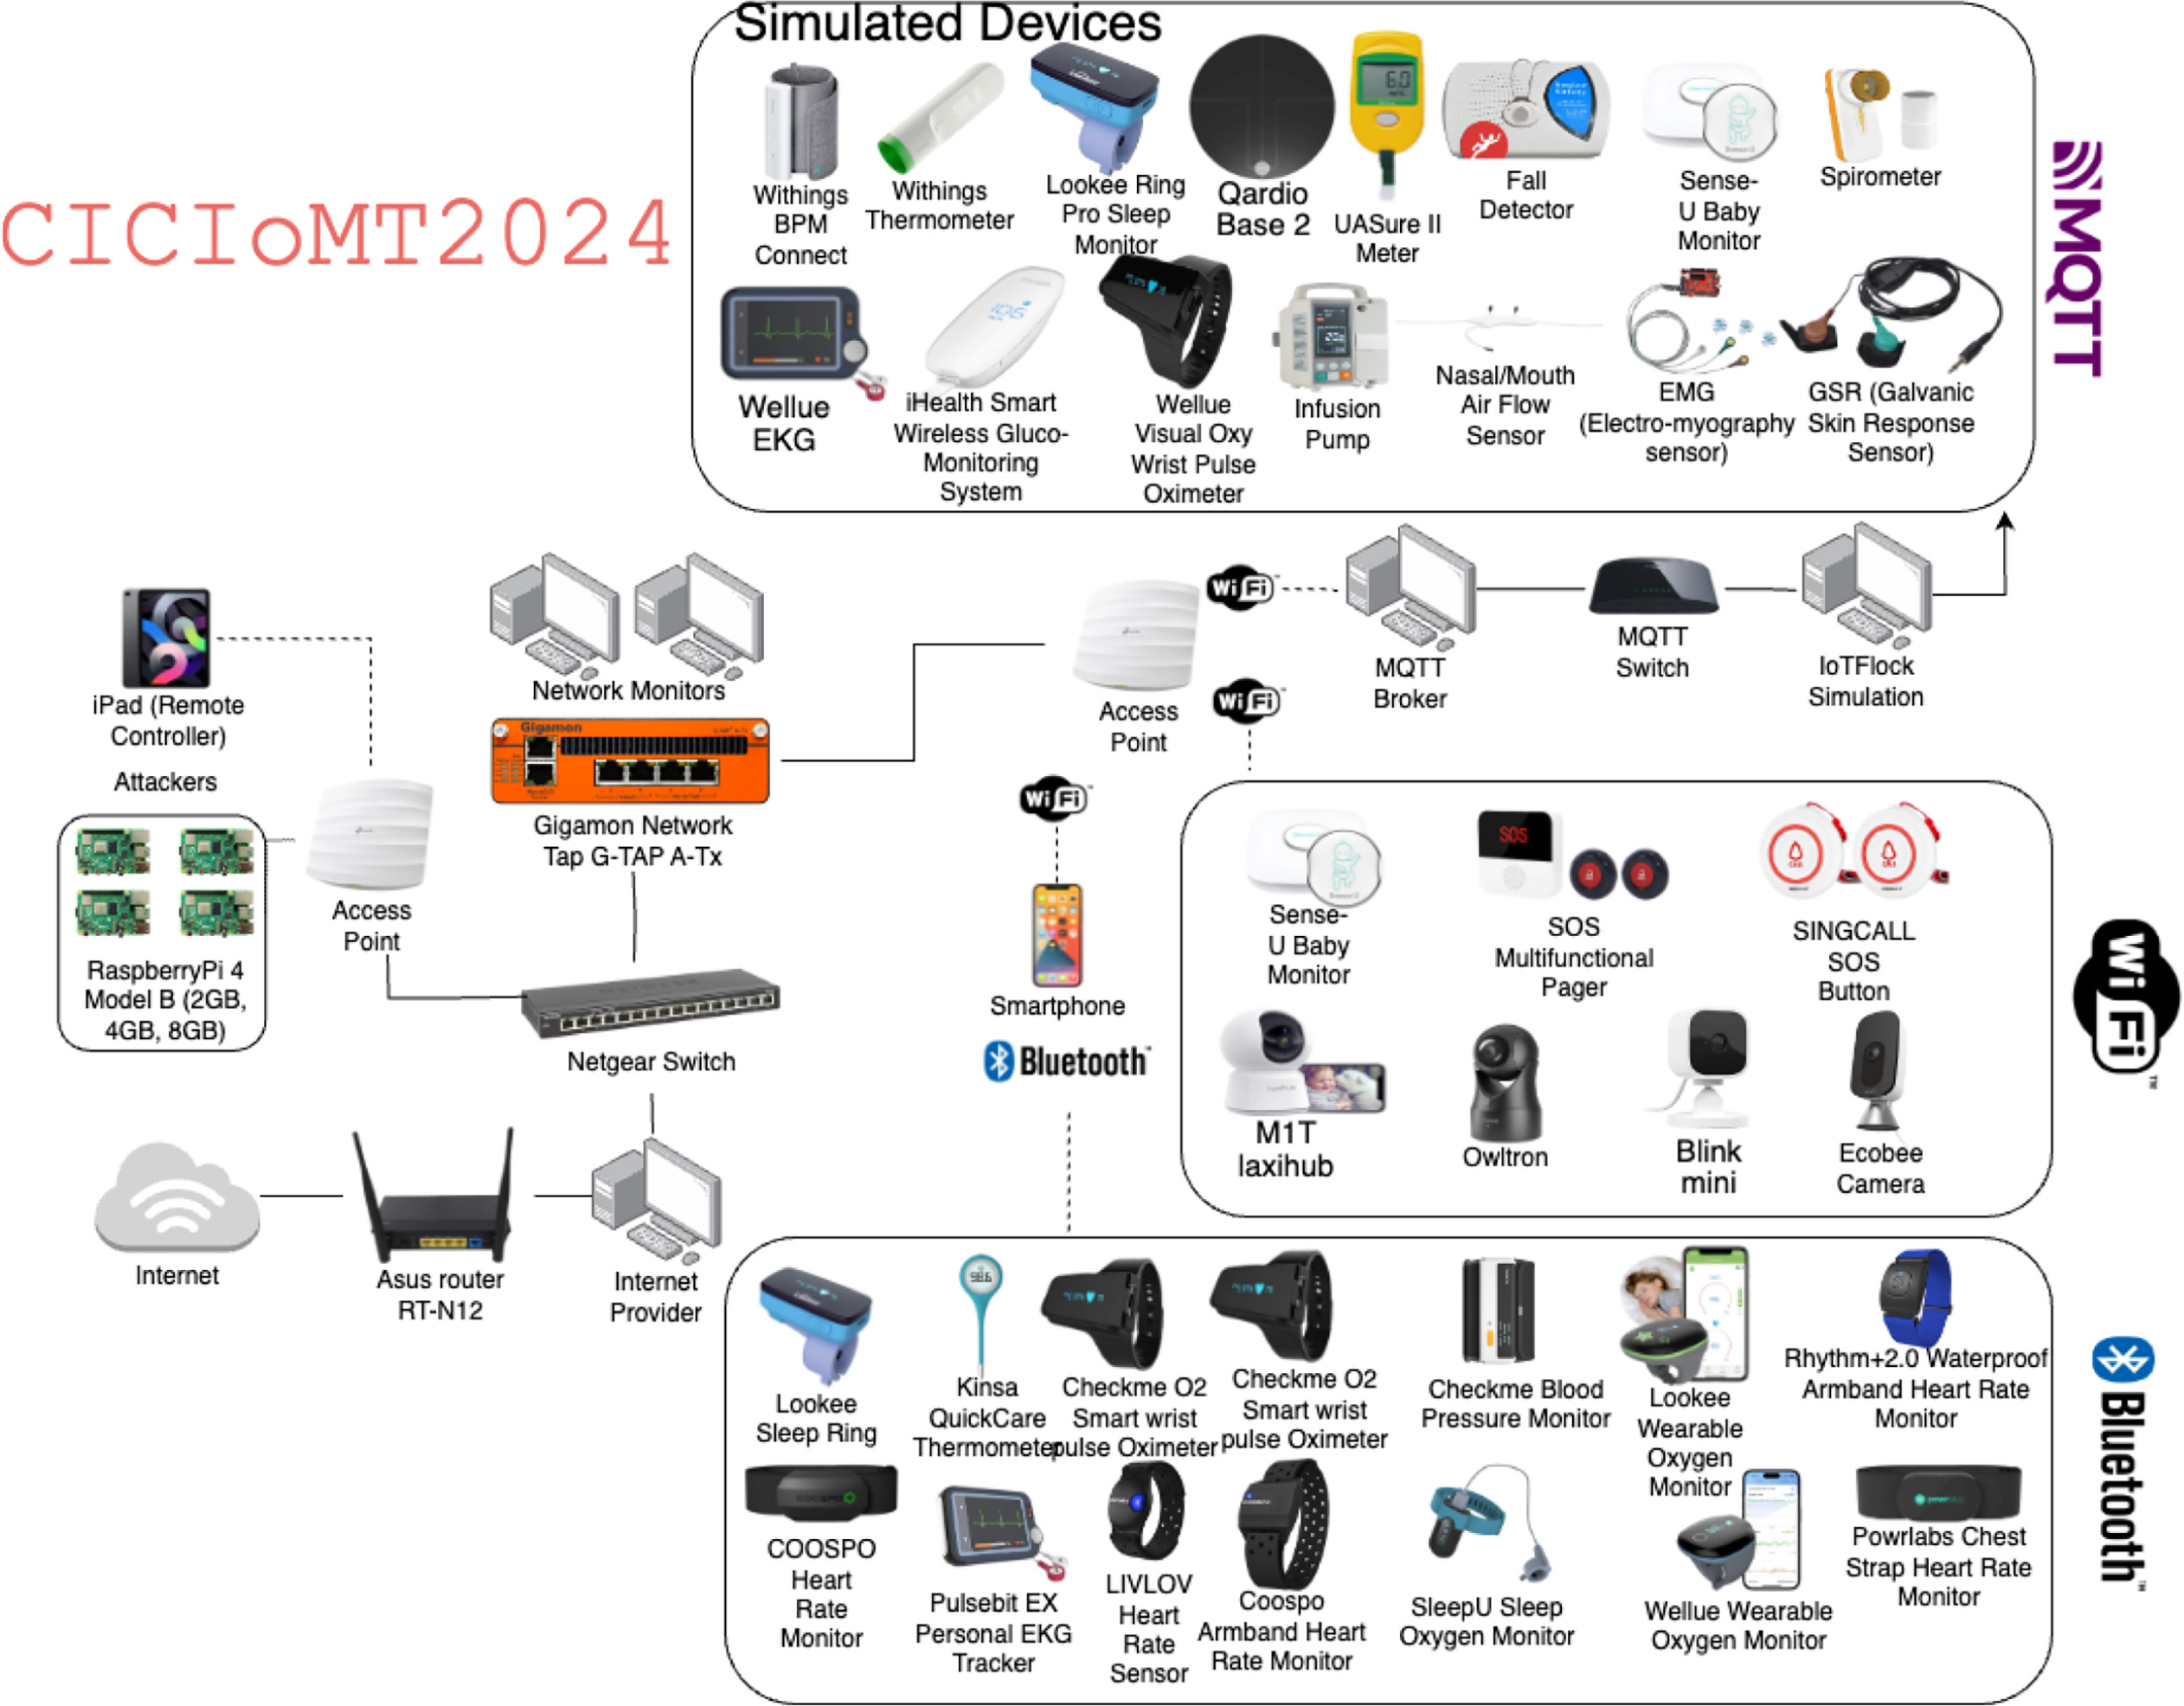
\includegraphics[width=0.7\textwidth]{./figures/fig-3.jpg}
  \caption{تجهیزاتی که موسسه کانادایی امنیت سایبری در اختیار محققان قرار داد.}
  \label{fig:cicIotLab}
\end{figure}

\subsubsection{توپولوژی شبکه دستگاه‌های \lr{IoMT}}

توپولوژی که محققان این پژوهش برای انجام آزمایشات خود راه‌اندازی کردند شامل
المان‌های زیر بوده است:

\begin{itemize}
    \item یک \lr{iPad} جهت کنترل فرایند‌ها و درخواست‌ها
    \item ۴ عدد \lr{RPi} که تمامی حملات از طریق آن‌ها انجام می‌شود.
    \item دستگاه‌های \lr{IoMT} که به وسیله یک \lr{Access point} به شبکه متصل
    هستند. با استفاده از این اتصال دستگاه‌های \lr{IoMT} می‌توانند به اینترنت
    دسترسی داشته باشند.
    \item تبادل داده‌ها بین دستگاه‌های \lr{IoMT} به گونه‌ای است که ۱۵، ۷ و ۱۴
    دستگاه به ترتیب با پروتکل‌های \lr{MQTT}، \lr{Wi-Fi} و بلوتوث ارتباط دارند.
\end{itemize}

\subsubsection{تولید ترافیک مخرب}

برای تولید ترافیک مخرب روی دستگاه‌های \lr{IoMT} از سناریو‌های واقعی در محیط‌های
مراقبت‌های بهداشتی استفاده شده است تا دیتاست کاملاً واقعی باشد. هدف این فرایند
ثبت ویژگی‌های ترافیک بدخیم و خراب‌کننده جهت تسهیل توسعه راهکار‌های امنیت سایبری
برای محیط‌های \lr{IoMT} می‌باشد. حملاتی که در این مرحله انجام شده عبارت‌اند از:

\begin{LTR}
    \begin{itemize}
        \item DoS
        \item DDoS
        \item ARP Spoofing
        \item Flooding campaings (Wi-Fi devices)
        \begin{itemize}
            \item ICMP
            \item SYN
            \item TCP
            \item UDP
        \end{itemize}
    \end{itemize}
\end{LTR}

\subsubsection{\lr{Wi-Fi}}

برای ایجاد ترافیک در این پروتکل ارتباطی، محققان حملات \lr{ARP Spoofing} را برای
\lr{Man in the middle} و بسیاری از حملات، \lr{TCP}، \lr{CYN}، \lr{ICMP} و
\lr{UDP} انجام دادند که همگی در دسته‌بندی \lr{DoS} و \lr{DDoS} قرار دارند.

\subsubsection{\lr{MQTT}}

در طی فعالیت‌ها در این پروتکل سه حمله انجام شده است:

\begin{itemize}
    \item \lr{MQTT Connect Flood}: در این حمله درخواست اتصال به \lr{Broker} با
    شدت زیاد ارسال می‌شود.
    \item \lr{MQTT Publish Flood}: ارسال بسته‌های مختلف به \lr{Topic}های مختلف و
    رندوم را انجام می‌دهد.
    \item \lr{MQTT Malformed Data Attack}: ارسال داده‌های نادرست را به
    \lr{Broker} برای تجزیه و تحلیل رفتار و جمع‌آوری اطلاعات \lr{Topic}های
    استفاده می‌کند.
\end{itemize}

در حمله آخر از ابزار \lr{MQTTSA} استفاده شد و سعی در \lr{Sniff} و شنود
\lr{Broker} با ارسال بسته‌های مشخص را داشتند تا رفتار دستگاه‌ها را بررسی کنند.
در این فرایند حمله، حمله‌کننده نام تمام تاپیک‌های \lr{MQTT} را که به صورت نهایی
منتشر شده‌اند را بدست می‌آورد و سعی می‌کند که به هر تاپیک داده نادرست را ارسال
کند. هدف اصلی این حملات بررسی و ارزیابی آسیب‌پذیری دستگاه‌های \lr{IoMT} در
پروتکل \lr{MQTT} بود. شبیه‌ساز با استفاده از ماشین مجازی \lr{VMware} که سیستم
عامل لینوکس اوبونتو نسخه $18.04.6$ راه‌اندازی شده بود و از نسخه \lr{GUI}
\lr{IoTFlock} که با زبان \lr{C++} نوشته شده بود مورد استفاده قرار گرفت.

\subsubsection{\lr{Bluetooth BLE 5.0}}

به طور کلی این ارزیابی برای بررسی مقاومت و تاب‌آوری دستگاه‌ها در برابر تهدیدات
امنیتی و اختلالات محیطی انجام شده است.

معمولاً حمله در بستر \lr{BLE} دو شرط الزامی را به همراه دارد:

\begin{enumerate}
    \item اجرای حمله
    \item جمع‌آوری ترافیک شبکه به روش‌ها و تکنیک‌های خاص
\end{enumerate}

فناوری \lr{BLE} به دلیل طراحی خاص خود که برای مصرف پایین انرژی بهینه شده است،
رفتاری متفاوت از پروتکل‌های بی‌سیم یا شبکه‌های معمولی دارد. بنابراین، اجرای
حملات یا ضبط ترافیک در این فناوری نیازمند ابزارها و تکنیک‌های متفاوتی است
\cite{matHackingTheBLE}. در این پژوهش، برای اجرای این حملات از یک تلفن همراه
هوشمند که به دستگاه \lr{BLE} متصل شده، استفاده شده است و سپس فعالیت‌های مخرب با
استفاده از کامپیوتر صورت گرفته است.

برای توسعه برنامه‌ای که قادر باشد تمامی بلوتوث‌های موجود در شبکه را جست‌وجو کند،
از کتابخانه \lr{Bleak} در زبان پایتون استفاده شده است. این برنامه توسعه‌یافته
می‌تواند به دستگاه‌های \lr{IoMT} متصل شده و تمامی سرویس‌ها و مشخصات آن‌ها را
دریافت کند. مشخصات دستگاه‌های \lr{IoMT} این امکان را فراهم می‌کند که دستگاه را
به شیوه‌ای خاص از عملکرد صحیح خود خارج کرد.

در ابتدا، برنامه بسته‌هایی با طول‌های مختلف ارسال می‌کند. طول هر بسته بین ۲۰ تا
۸۱۰ بایت، با افزایش ۱۰ بایتی تنظیم شده است. داده‌های ارسالی به شکل الگوی تکراری
مانند $01234567890123456\ldots$ هستند که اعداد به صورت پشت سر هم تکرار می‌شوند.
هر بار که ارسال موفقیت‌آمیز انجام می‌شود، لاگ مربوطه ثبت می‌گردد. سپس برنامه
مشخص می‌کند که هر بسته با موفقیت روی کدام \lr{UUID} ارسال شده است.

آدرس \lr{UUID} که مشابه \lr{SSID} در شبکه‌های بی‌سیم \lr{Wi-Fi} است، برای مشخص
کردن آدرس شبکه بلوتوث استفاده می‌شود. پس از این مرحله، برنامه وارد حلقه‌ای
می‌شود که داده‌ها روی \lr{UUID}های شناسایی‌شده ارسال می‌شوند و در نهایت در یک
متغیر ذخیره می‌گردند. این ارسال‌های پی‌درپی به منظور ایجاد بار اضافی
(\lr{Overload}) در دستگاه انجام می‌شوند که منجر به اختلال در عملکرد صحیح دستگاه
شده و حمله‌ای شبیه به \lr{DoS} را شبیه‌سازی می‌کند.

داده‌ها به دو روش جمع‌آوری می‌شوند. در روش اول، لاگ‌های سمت دستگاه اندروید که به
دستگاه \lr{IoT} متصل است، بررسی می‌شوند. روش دوم شامل استفاده از \lr{Sniff} شبکه
بلوتوث با استفاده از برد \lr{Ubertooth} است که از طریق کامپیوتر متصل شده و
قابلیت شناسایی تمامی بلوتوث‌های موجود در محدوده را فراهم می‌کند.

هدف اصلی از تحلیل این دو نوع لاگ، دستیابی به یک درک جامع و کلان از رفتار
دستگاه‌ها در حالت عادی و هنگام وقوع حمله است. این حملات به شکل‌های مختلف آنقدر
تکرار می‌شود تا نتیجه‌اش را به عنوان بررسی انعطاف‌پذیری و آسیب‌پذیری دستگاه در
بستر حمله‌های مبتنی بر \lr{BLE} ثبت کنند.

دستگاه‌های \lr{IoMT} که در این حمله شرکت داشته‌اند به صورت زیر می‌باشد که هر
کدام رفتار متفاوتی را نسبت به حملات داشته‌اند:

\begin{table}[h!]
    \centering
    \begin{tabular}{|l|p{10cm}|}
        \hline
        \textbf{نام دستگاه} & \textbf{نتیجه بررسی} \\ \hline
        \lr{Lookee Sleep Ring} & بدون وقفه عملکرد دستگاه در طی حملات مورد تأیید قرار گرفت. \\ \hline
        \lr{Powerlabs HR Monitor Arm Band} & دستگاه باید طبق استانداردها، حتی تحت حمله عملکرد صحیح خود را داشته باشد. \\ \hline
        \lr{COOSPO HW807 Armband} & حملات منجر به ایجاد اختلال و خاموش شدن دستگاه شدند که نشان‌دهنده شکست سخت‌افزار در برابر عوامل خارجی است. \\ \hline
        \lr{Livlov Heart Rate sensor} & سنسور بدون وقفه در برابر حملات مقاومت کرد. \\ \hline
        \lr{Wellue O2 Ring} & دستگاه بدون وقفه به عملیات خود ادامه داد. \\ \hline
        \lr{Lookee O2 Ring} & دستگاه تحت تأثیر حملات دچار اختلال شدید شد و خاموش شد. \\ \hline
        \lr{Checkme BP2A} & دستگاه داده‌ها را فقط در صورت اتصال پایدار بلوتوث ارسال می‌کرد، که نشان‌دهنده طراحی ایمن برای حفظ امنیت داده‌ها است. \\ \hline
        \lr{SleepU Sleep Oxygen Monitor} & در برابر حملات مقاومت کرده و بدون وقفه عمل کرده است. \\ \hline
        \lr{Rhythm+2.0 (Scosche)} & دستگاه به شدت تحت تأثیر حمله قرار گرفت و خاموش شد. \\ \hline
        \lr{Wellue Pulsebit EX} & دستگاه در برابر حملات مقاومت کرد و بدون قطعی به عملیات خود ادامه داد. \\ \hline
        \lr{Checkme O2 Smart Pulse Oximeter} & دستگاه مقاومت کرده و به عملیات استاندارد خود ادامه داده است. \\ \hline
        \lr{Kinsa Thermometer} & تحت تأثیر حملات قرار گرفت و تنها راه ریست کردن اتصال، تخلیه باتری بود. \\ \hline
        \end{tabular}
        \caption{نتایج بررسی دستگاه‌ها تحت حملات مختلف}
    \label{table:attack_results}
\end{table}

لازم به ذکر است که تمام حملات صورت گرفته کاملاً در محیطی ایزوله از هر گونه
سیگنال خارجی انجام شده است تا با ترافیک شبکه جمع‌آوری شده هیچ سیگنال مزاحمی
وجود نداشته باشد.

\subsection{\lr{IoMT profiling}}

درک کامل جنبه‌های مختلف رفتار عملیاتی دستگاه‌های \lr{IoMT} برای بهبود امنیت سیستم
بسیار حیاتی است. ارزیابی پروفایل‌های \lr{IoMT} قابلیت کلاسیفایرها را در تشخیص
ناهنجاری‌های عملکردی دستگاه‌های مراقبت بهداشتی تقویت کرده و امکان تمایز بین
رفتار عادی و غیرعادی شبکه را فراهم می‌سازد. در تسک‌هایی که کلاسیفای نشده‌اند،
الگوهای مشاهده‌نشده می‌توانند نشان‌دهنده فعالیت‌های مخرب و حملات zero-day باشند.

حملات \lr{zero-day} به نوعی حمله سایبری اشاره دارند که از یک آسیب‌پذیری ناشناخته
یا به‌تازگی کشف‌شده در نرم‌افزار، سخت‌افزار یا سیستم بهره می‌برند. نام این نوع
حمله از آنجا گرفته شده است که توسعه‌دهنده یا مالک سیستم پیش از وقوع حمله
برنامه‌ای برای شناسایی و رفع آسیب‌پذیری نداشته است. در این تحقیق، تمامی حملات
موردنظر شبیه‌سازی و بررسی شده‌اند تا توسعه‌دهندگان و شرکت‌ها بتوانند از قرار
گرفتن در معرض حملات \lr{zero-day} جلوگیری کنند.

ویژگی‌های اصلی حملات \lr{zero-day} \cite{enwiki:1268124149}:

\begin{itemize}
    \item آسیب‌پذیری ناشناخته: آسیب‌پذیری که هنوز توسط تیم امنیتی یا تیم توسعه
    کشف یا رفع نشده است.
    \item غالفگیری: به دلیل آگاهی از آسیب‌‌پذیری، سیستم‌ها در برابر این نوع
    حملات کامل آسیب‌پذیر هستند.
    \item سوء استفاده یا \lr{Exploit}: مهاجمان معمولاً از کد یا تکنیک‌هایی برای
    بهره‌برداری از آسیب‌پذیری استفاده می‌کنند.
\end{itemize}

\subsubsection{آزمایش‌های مبتنی بر انرژی و باتری}

آزمایش‌های این قسمت مربوط به مصرف انرژی دستگاه‌های مجهز به \lr{Wi-Fi} بوده است.
این آزمایش‌ها تلاش می‌کنند تا رفتار دستگاه‌های \lr{Wi-Fi} را از نظر مصرف انرژی و
ارسال داده‌ها در هنگام روشن و یا خاموش بودن را به دقت تحلیل کنند. این آزمایش
تنها روی هفت دستگاه \lr{Wi-Fi} تمرکز دارند و روی دستگاه‌های \lr{MQTT} شبیه‌سازی
نشده‌اند. برای انجام این آزمایش:

تمام دستگاه‌ها از شبکه خارج شده‌اند و به جایی متصل نخواهند بود. تنها دستگاه متصل
به شبکه یک دستگاه \lr{iPad} خواهد بود که برای کنترل و نظارت بر سایر دستگاه
استفاده می‌شود. حتی دستگاه‌های \lr{RPi} نیز در این آزمایش متصل نبودند. مراحل زیر
در ادامه انجام شده‌اند:

\begin{enumerate}
    \item در مرحله اول، دستگاه مورد نظر روشن شد و رفتار آن برای مدت ۲ دقیقه با
    استفاده از فیلتر آدرس \lr{MAC} ثبت شد.
    \item در مرحله دوم، دستگاه خاموش می‌شود و فرایند ثبت داده‌ها برای ۳ دقیقه
    دیگر ادامه پیدا می‌کند تا هر بسته اطلاعاتی باقی‌مانده شناسایی شوند و اطمینان
    حاصل شود که دیگر هیچ بسته‌ای ارسال نمی‌شود.
\end{enumerate}

فرایند انجام شده بالا دقیقاً همانند فرایندی است که در جمع‌آوری دیتاست
\lr{CICIoT2021} انجام شده بود. نکته قابل توجه آن است که برخی از دستگاه‌ها کلید
روشن و خاموش نداشتند و برای انجام آزمایش نیاز به انجام تنظیمات مخصوص داشتند:

\begin{LTR}
    \begin{itemize}
        \item Singcall Sensor
        \item SOS Multifunctional Page
        \item Sense U Baby
    \end{itemize}
\end{LTR}

\subsubsection{آزمایشگاه‌های مبتنی بر حالت \lr{Idle}}

آزمایشاتی است که تنها در زمان روشن بودن دستگاه ولی در حالی که هیچ داده‌ای منتقل
نمی‌کردن، انجام می‌شود. انجام این آزمایش به محققان اجازه داد که رفتار حالت عادی
و \lr{baseline} شبکه رو بهتر متوجه بشن. در این آزمایش ۱۳ ساعت عملیات بررسی و
آزمایش طول کشید. آزمایشات بین دو شب از ساعت ۶ عصر تا تا ۷ صبح برای اطمینان از
اینکه هیچ تعاملی دستگاه‌ها ندارند انجام شد.

\subsubsection{آزمایش‌های فعال}

شامل دستگاه‌هایی می‌شود که وظایف مورد نظر خود را انجام می‌دادند و ترافیک عادی را
در شبکه بابت عملیات خود ایجاد می‌کردند.

\subsubsection{آزمایش‌های مبتنی بر تعامل}

این قسمت از آزمایشات روی تعامل با دستگاه‌ها متمرکز است که به صورت زیر انجام
شده‌اند:

\begin{itemize}
    \item فیزیکی: کاربر مستقیماً با دستگاه ارتباط برقرار می‌کند.
    \item دیجیتالی:‌برنامه‌ها بایکدیگر ارتباط می‌گیرند و ارسال داده انجام
    می‌دهند.
\end{itemize}

سه نوع تعامل بررسی شده است:

\begin{itemize}
    \item تعامل فیزیکی:
    \begin{itemize}
        \item این آزمایشات زمانی انجام شده‌اند که دستگاه‌ها دارای دکمه فیزیکی
        بوده‌اند.
        \item آزمایشات با ترکیب تعامل فیزیکی و شبکه‌های محلی یا شبکه‌های گسترده
        صورت گرفته است:
        \begin{itemize}
            \item در شبکه محلی: اپلیکیشن و دستگاه در یک شبکه قرار دارند.
            \item در شبکه \lr{WAN}: اپلیکیشن از شبکه‌ای متفاوت نسبت به دستگاه
            متصل بوده است.
        \end{itemize}
    \end{itemize}
    \item تعامل در شبکه محلی:
    \begin{itemize}
        \item در این آزمایشات از اپلیکیشن‌های همراه دستگاه استفاده شده است.
        اپلیکیشن و دستگاه هر دو در یک شبکه با استفاده از \lr{Wi-Fi} بوده‌اند.
        برای مثال روشن و خاموش کردن دستگاه از طریق اپلیکیشن در خانه.
        \item در تعامل با شبکه گسترده نیز همینطور بوده است، اپلیکیشن همراه
        دستگاه به شبکه‌ای متفاوت متصل بوده و کنترل دستگاه از راه دور مثلاً روشن
        کردن دستگاه خانه از دفتر کار صورت گرفته است.
    \end{itemize}
\end{itemize}

\subsection{ارزیابی‌های مبتنی بر یادگیری ماشین}

آزمایشاتی که انجام شده آنقدر باعث تولید داده شد که می‌توان با استفاده از آن‌ها
ارزیابی‌هایی را برای تشخیص و جلوگیری حمله در سیستم‌های \lr{IoMT} انجام داد. از
جمله این مدل‌های یادگیری ماشین می‌توان به موارد زیر اشاره کرد:

\begin{LTR}
    \begin{itemize}
        \item Logistic Regression
        \item Random Forest
        \item Adaboost
        \item Deep Neural Networks (DNN)
    \end{itemize}
\end{LTR}

دسته‌بندی و طبقه‌بندی داده‌ها نیز می‌تواند به صورت \lr{attack} و \lr{Benign} یا
به صورت مشخص‌تر، \lr{Dos, MQTT, recon} و یا \lr{DDoS} انجام شود.
\section{رابطه مدل‌های ریاضی با شاخص‌های کلیدی کارایی}

از پژوهش \cite{vcolakovic2023iot} درک می‌کنیم که برای مدل‌سازی جهت ارزیابی
عملکرد سیستم‌های مختلف از قبیل سیستم‌های \lr{IoT} بایستی شاخص‌های کلیدی کارایی
یا \lr{KPI} \footnote{\lr{Key Performance Indicators}} را بشناسیم. این
\lr{KPI}ها شامل مجموعه‌ای از فرمول‌های ریاضیاتی هستند که نسبت به نیازمندی‌های
غیرعملیاتی یا \lr{Non-functional requirements} متفاوت می‌باشند. نیازمندی‌های
غیرعملیاتی مانند میزان مصرف انرژی، میزان مصرف حافظه، سرعت انتقال اطلاعات و
گذردهی، میزان دقت، میزان دردسترس بودن، میزان قابلیت اطمینان و غیره می‌باشد. برای
هر کدام از این نیازمندی‌های غیرعملیاتی فرمول‌هایی وجود دارد که می‌تواند با
فراگیری آن‌ها به مقادیری رسید که در مرحله بعد می‌توان آن‌ها را در مدل‌های
ریاضیاتی استفاده کرد.  مرحله دوم در حقیقت ارزیابی کارایی سیستم‌ها با استفاده از
مدل‌های شناخته شده ریاضیاتی می‌باشد که رابطه مستقیمی با \lr{KPI}‌ها دارند. یعنی
‌نمی‌توان مقادیر \lr{KPI} را برای این مدل‌ها نادیده گرفت. در نهایت با مدل‌های
مطرح شده می‌توان کارایی سیستم‌های \lr{IoT} در دامنه‌های مختلف را ارزیابی کرد و
بین آن‌ها مقایسه و \lr{Trade off} نسبت به \lr{Benchmark}های بدست آمده انجام داد.
مجموعه‌ای از مفاهیم جدید در حوزه پردازش مطرح شده‌اند که کاربردهای متنوعی در
استفاده از اینترنت اشیا (\lr{IoT}) دارند. این مفاهیم شامل \lr{Fog Computing}،
\lr{Edge Computing}، \lr{Mobile Edge Computing}، \lr{Mobile Cloud Computing} و
\lr{Cloudlet} ‌ها هستند. در این مقاله، یک مدل ریاضیاتی برای توصیف رسمی سیستم‌های
\lr{IoT} ارائه شده است. علاوه بر این، ارزیابی دقیقی از طراحی این سیستم‌ها با
توجه به معماری، تکنولوژی‌ها، پروتکل‌ها و مدل‌های یکپارچه‌سازی برای بهینه‌سازی
عملکرد ارائه شده است. مطالعه این مقاله ما را با یک روش بهینه برای بهبود کارایی
سیستم‌های مبتنی بر فرآیندهای \lr{offloading} مانند \lr{load balancing} آشنا
می‌کند.

\lr{KPI}ها و مدل‌هایی که در این گزارش مورد بررسی قرار گرفته‌اند:

\subsection{\lr{KPI}ها}

\begin{itemize}
    \item فرمول شانون
    \item فرمول محاسبه \lr{System load}
    \item فرمول تاخیر سرویس‌دهی یا \lr{Service latency}
    \item مصرف انرژی
\end{itemize}

\subsection{مدل‌ها}

\begin{itemize}
    \item تابع سودمندی یا \lr{Utility function}
    \item فرمول تابع سیگموئید
\end{itemize}

\subsection{چالش سیستم‌های جدید}

یکپارچه‌سازی سیستم‌های \lr{IoT} با سیستم‌های مختلف مانند سیستم‌های \lr{Cloud} و
\lr{Fog} چالش‌های زیادی را به همراه داشته است، مانند:

\begin{itemize}
    \item تاخیر‌های شبکه‌ای
    \item گذردهی
    \item مصرف انرژی
    \item قابلیت اطمینان
\end{itemize}

\subsection{مزیت مدل‌سازی سیستم‌های \lr{IoT}}

مدل‌سازی ریاضیاتی سیستم‌های \lr{IoT} نمایی کلی از سیستم را ارائه می‌دهد که به
درک بهتر عناصر، تعاملات، و رفتارهای آن‌ها کمک می‌کند:

\begin{enumerate} 
    \item مدل مفهومی یا \lr{conceptual model}: ساختاری سطح بالا برای توصیف
    عملیات‌هایی که در سیستم‌های \lr{IoT} انجام می‌شود. 
    \item مدل رفتاری یا \lr{behavioral model}: این مدل ممکن است شامل جزئیاتی
    مانند جریان داده بین المان‌ها باشد. 
\end{enumerate}

به طور کلی، مدل‌سازی به شناسایی و پاسخ به مسائل مربوط به کارایی کمک شایانی
می‌کند و امکان بهینه‌سازی، کارایی بیشتر و اطمینان از عملکرد بهتر سیستم‌ها را
فراهم می‌آورد.

هر زمان که درباره مدل‌سازی یک سیستم \lr{IoT} صحبت می‌شود، هدف ایجاد چهارچوبی است
که بتوان با استفاده از آن سیستم را تست، اعتبارسنجی (\lr{validation}) و یا برای
پاسخگویی به تقاضاها بهینه‌سازی کرد.

\subsection{طبقه‌بندی \lr{IoT} در دامنه‌های متفاوت}

فرآیندهای سیستم‌های \lr{IoT} معمولاً شامل شناسایی، دریافت اطلاعات
(\lr{Sensing})، فعالیت‌های مبتنی بر شبکه، و محاسبات کوچک هستند که امکان ارتباط
با محیط فیزیکی و اشیاء مختلف را فراهم می‌کنند.

در این مقاله سیستم‌های \lr{IoT} با کاربردی که دارند به ۴ دسته تقسیم می‌شوند:

\begin{figure}[H]
  \centering
  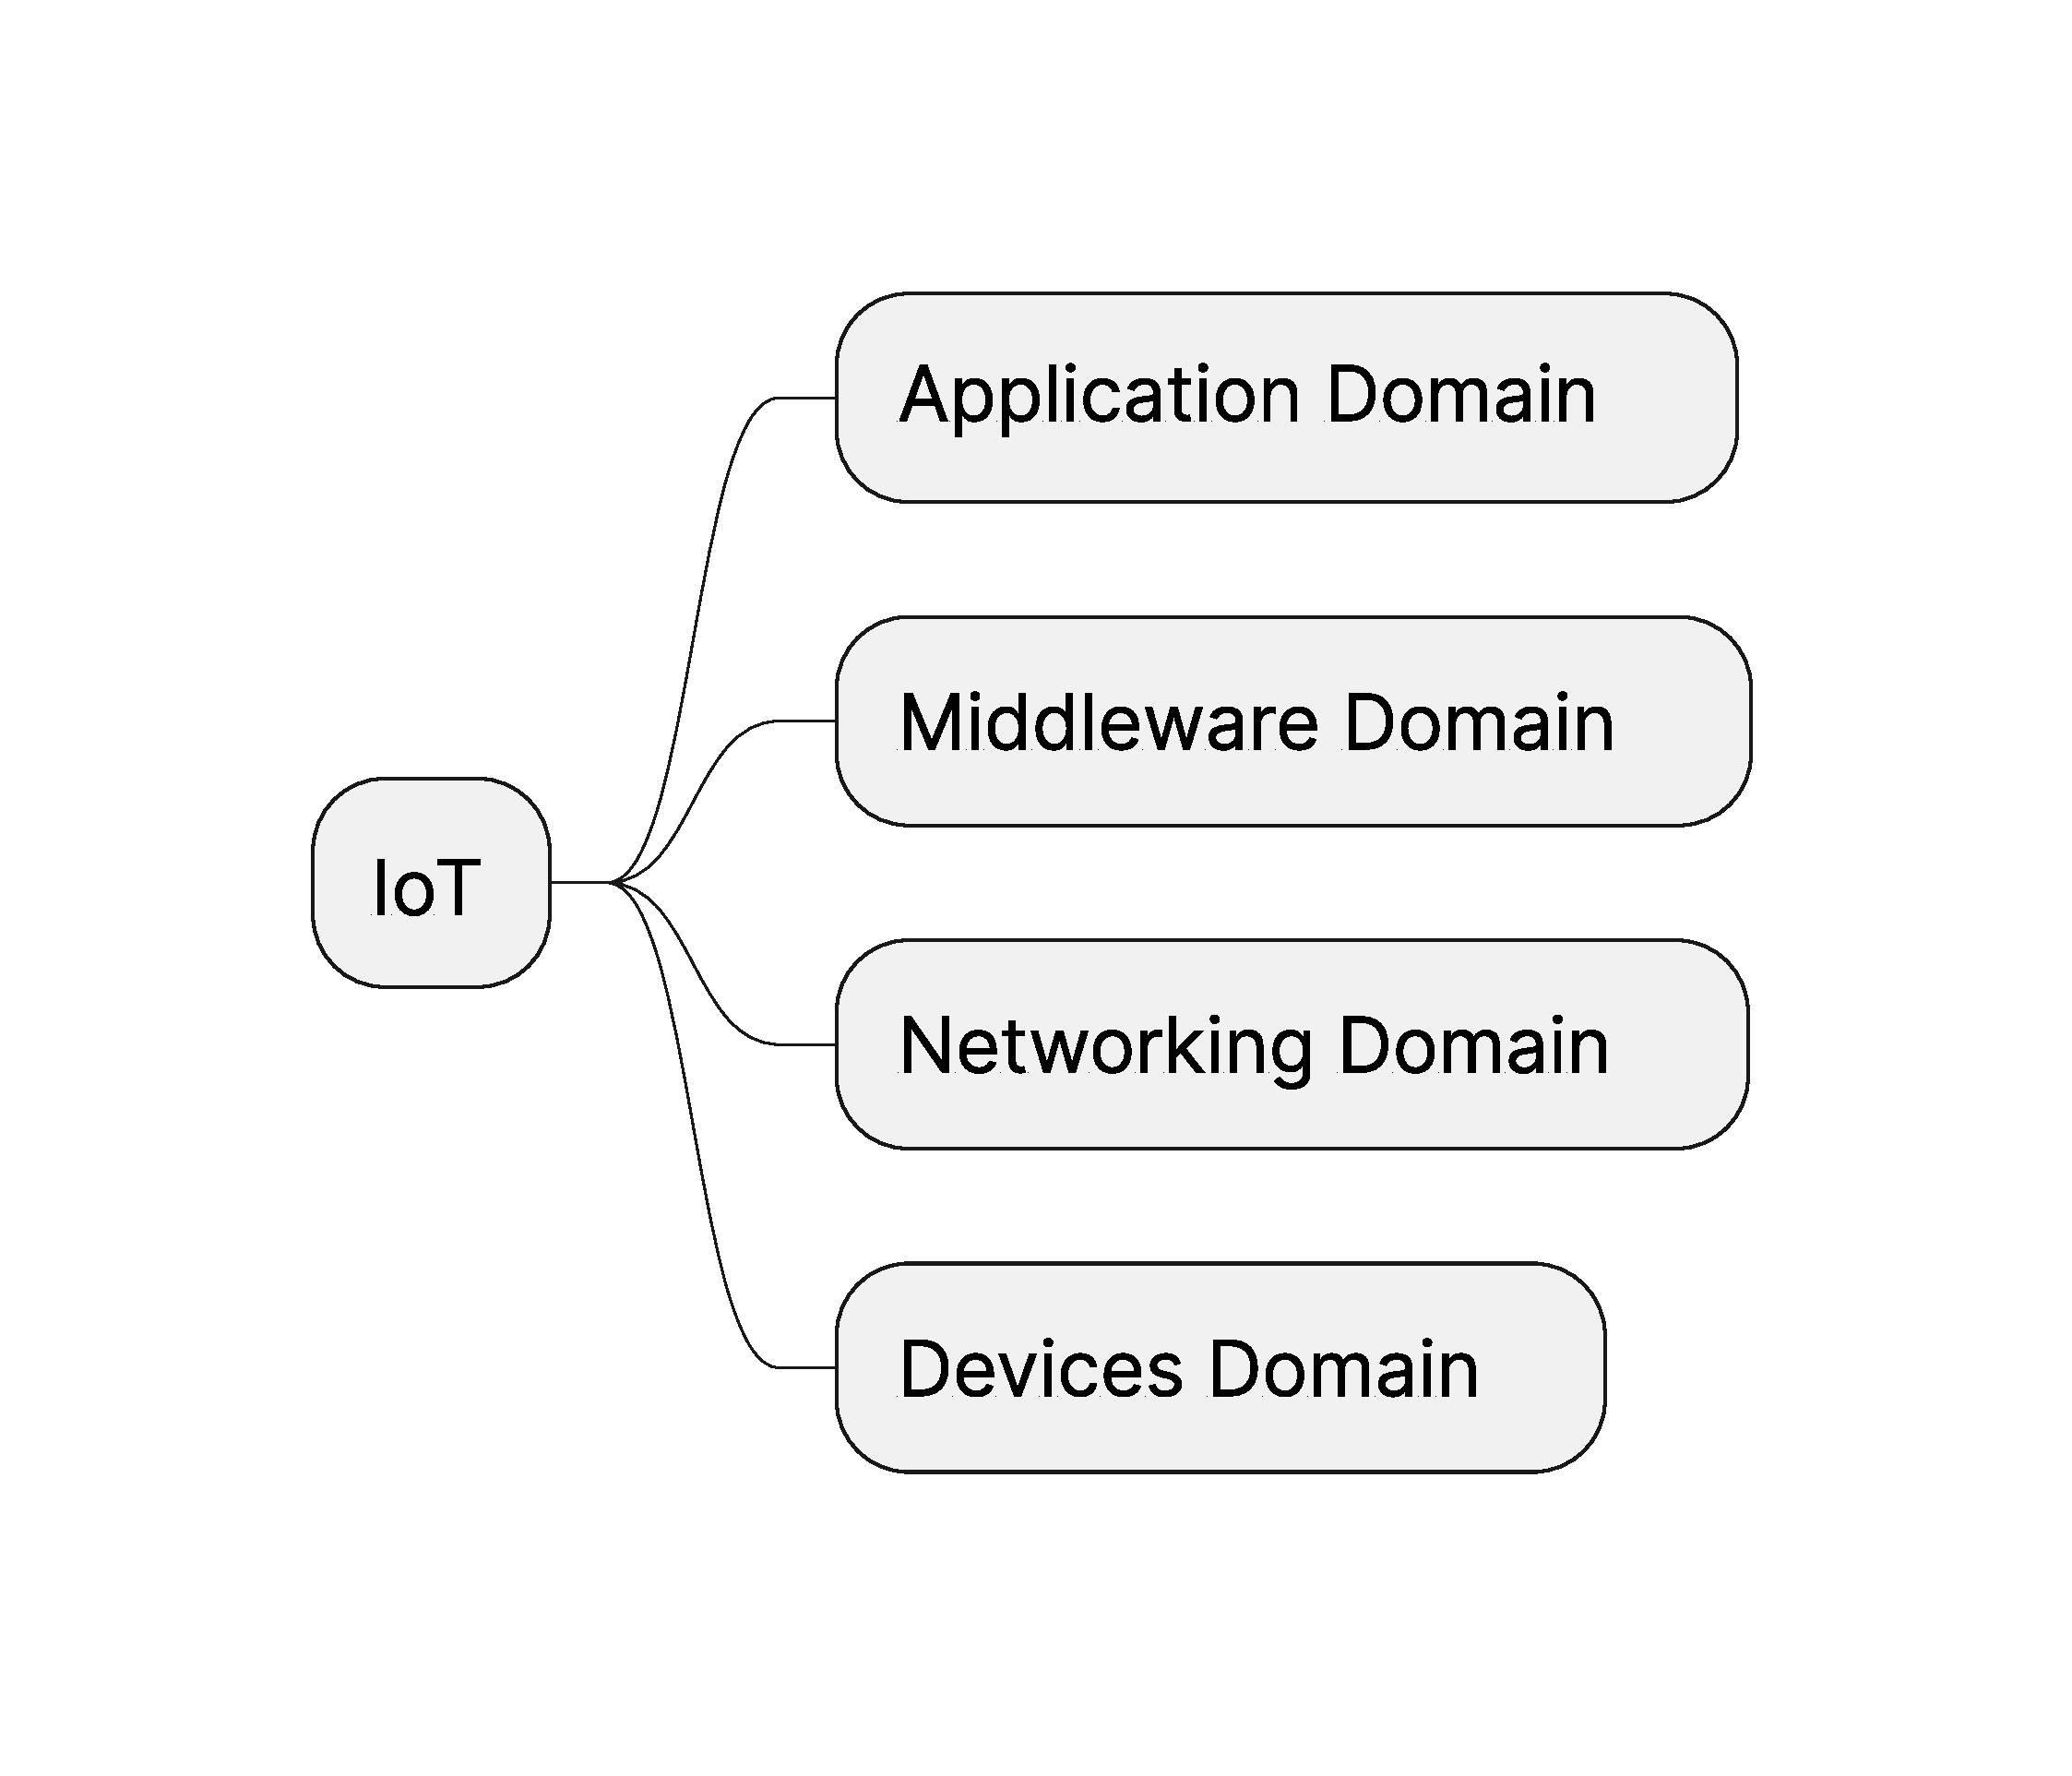
\includegraphics[width=0.6\textwidth]{./figures/IoT_overall_domains.pdf}
  \caption{۴ دسته‌بندی دامنه استفاده از سیستم‌های \lr{IoT}}
  \label{fig:iotOverallDomains}
\end{figure}

\begin{figure}[H]
  \centering
  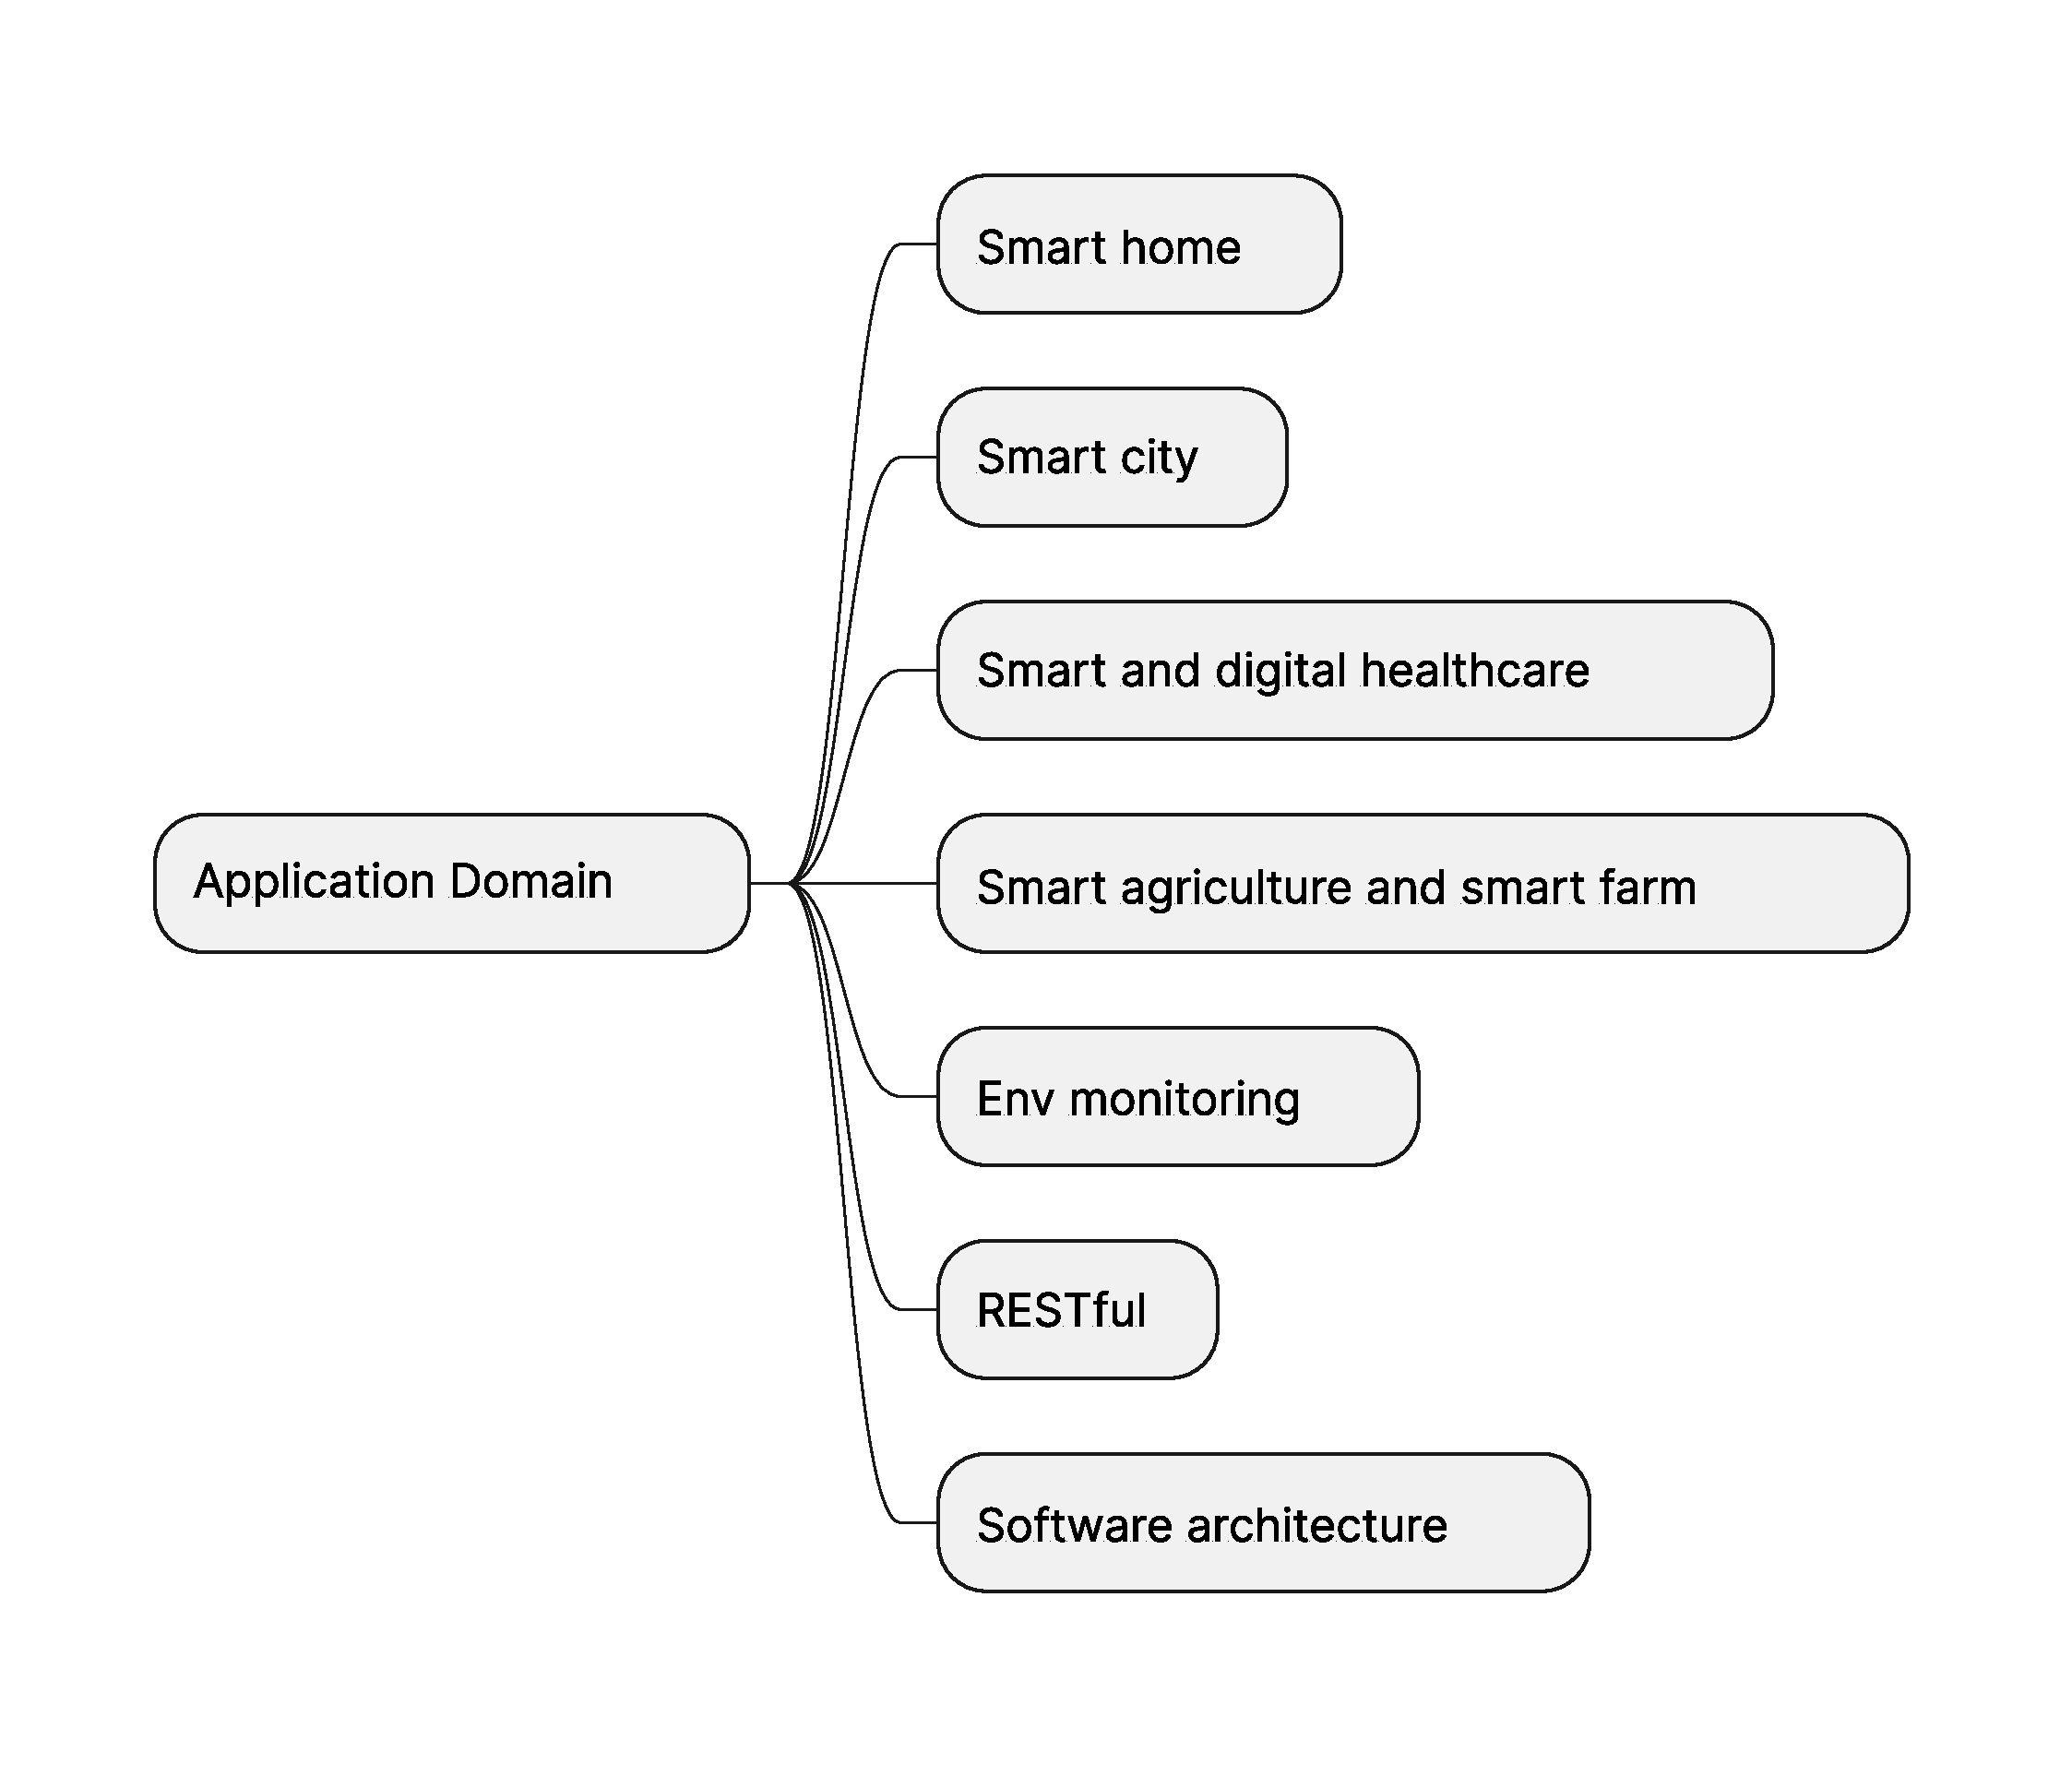
\includegraphics[width=0.9\textwidth]{./figures/IoT_application_domains.pdf}
  \caption{حوزه‌های تخصصی بخش اپلیکیشن در \lr{IoT}}
  \label{fig:iotApplicationDomains}
\end{figure}

\begin{figure}[H]
  \centering
  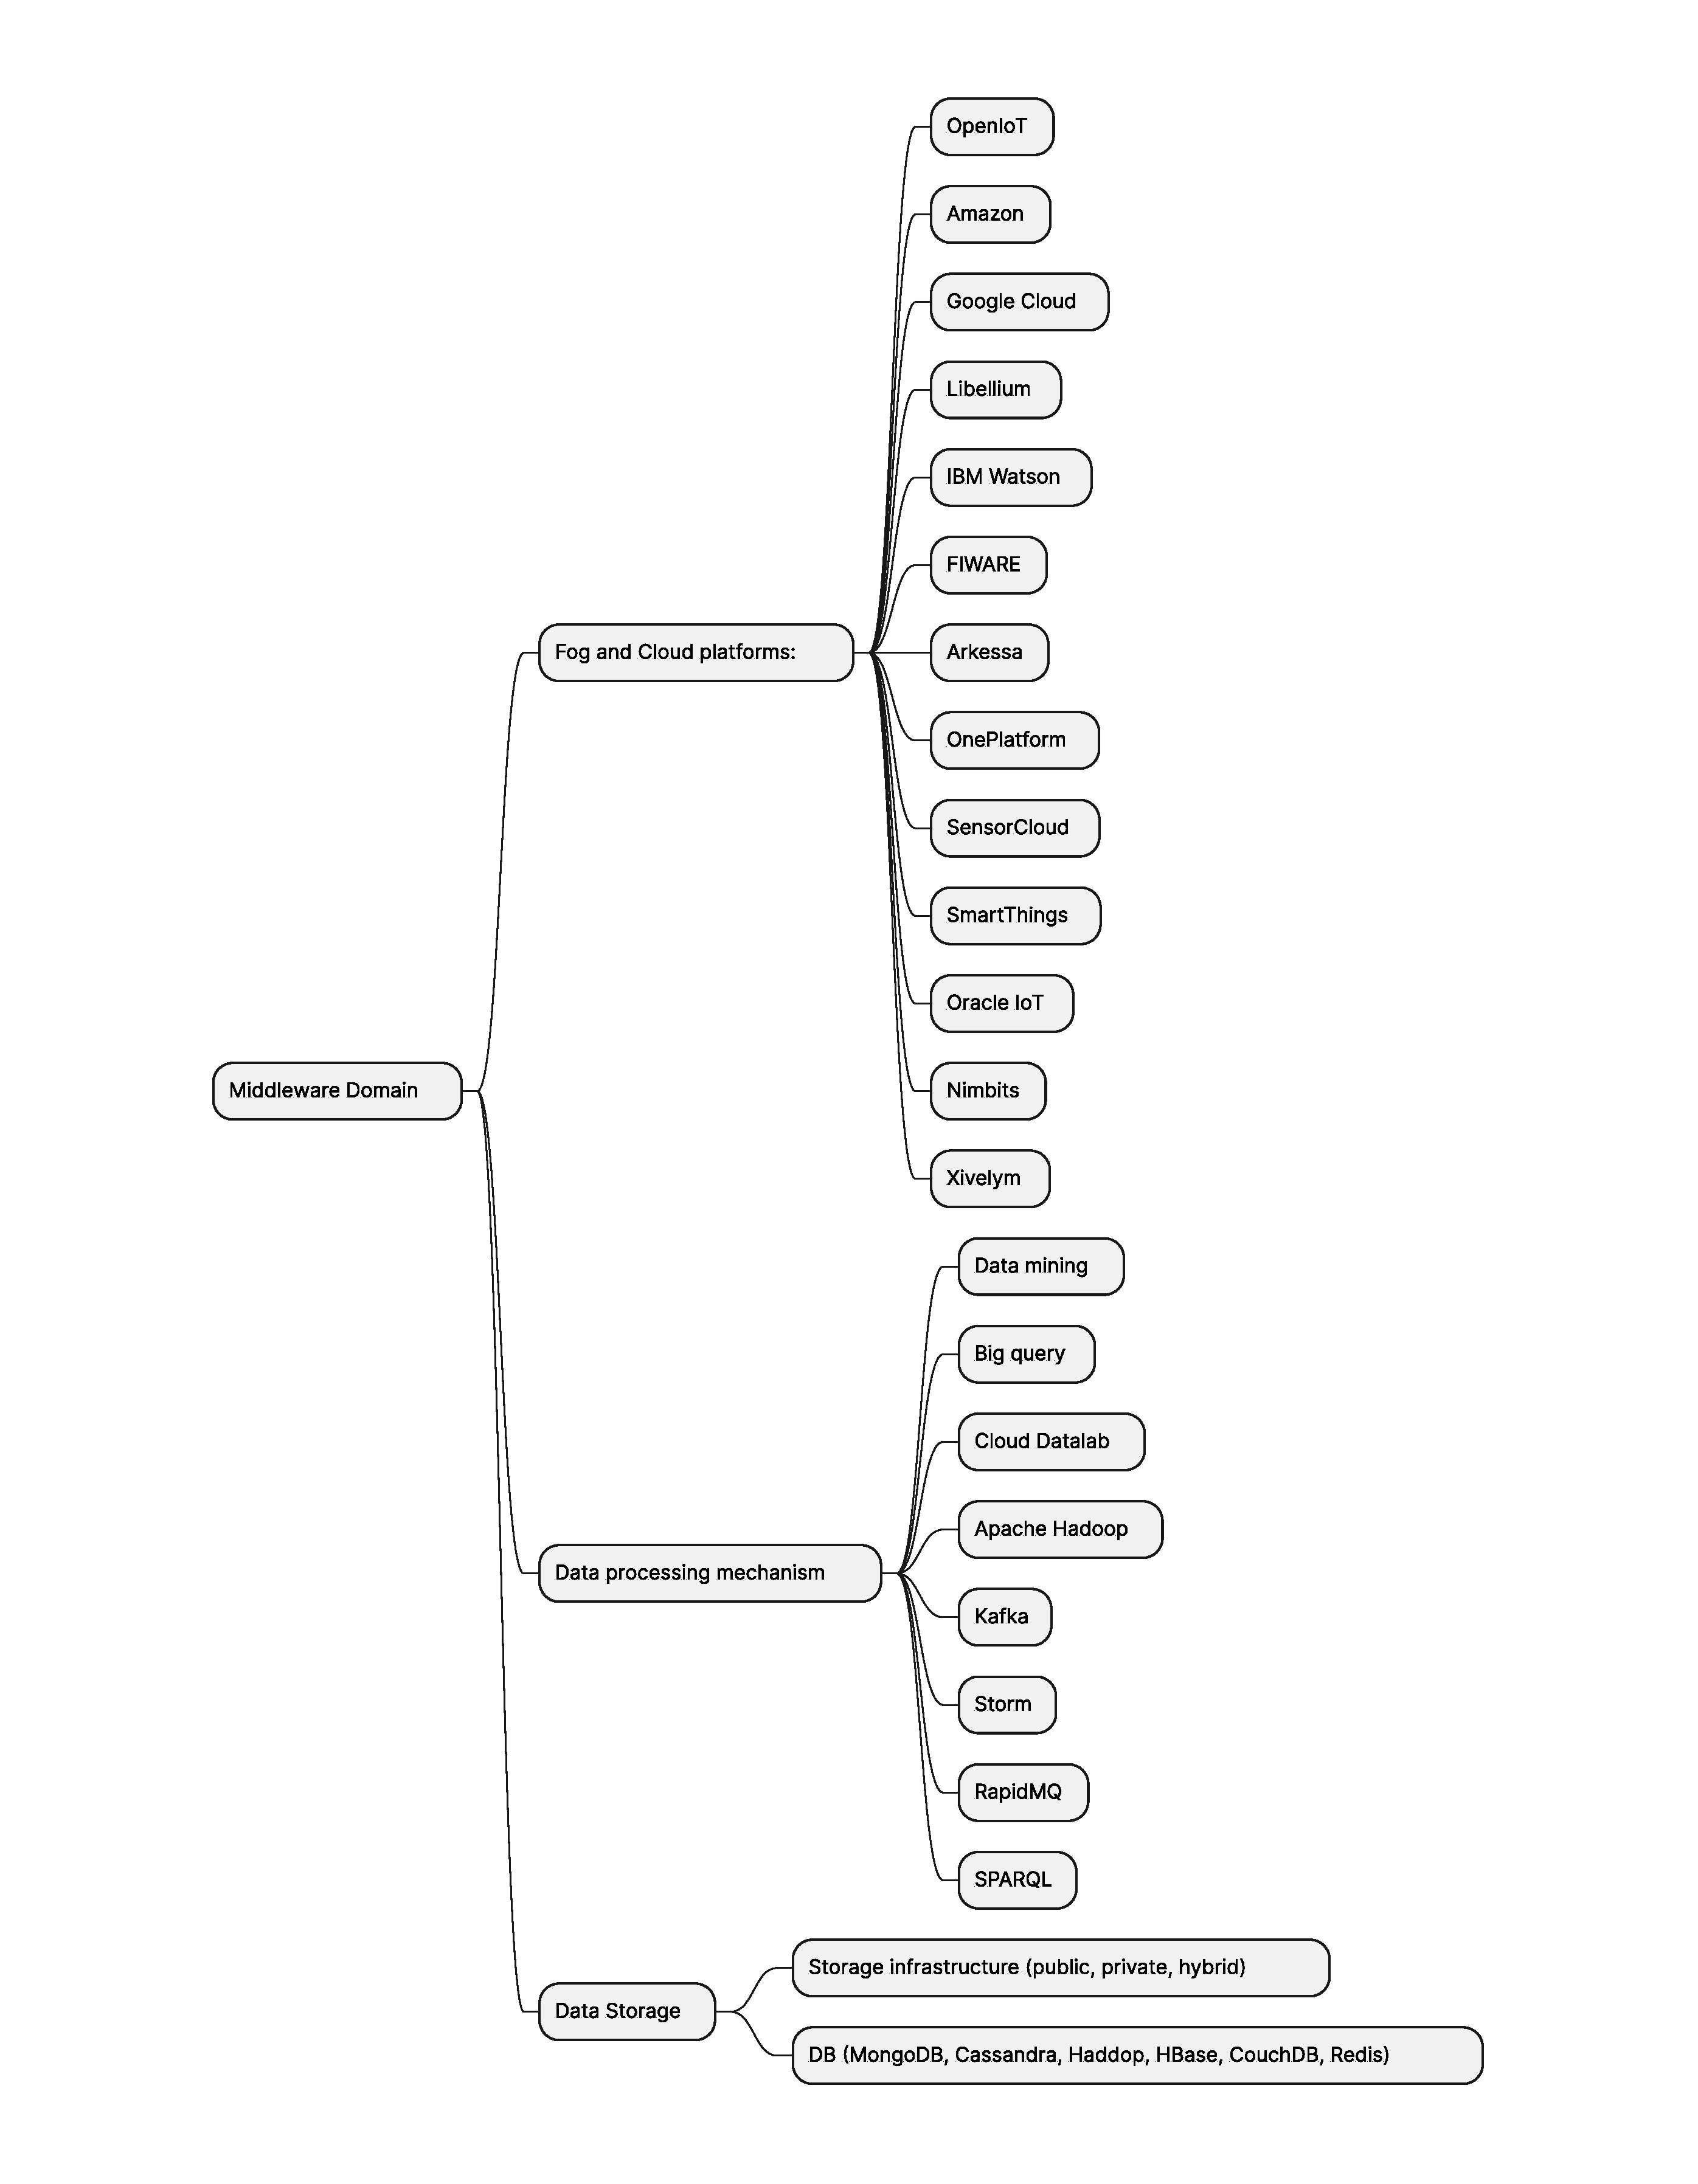
\includegraphics[width=0.9\textwidth]{./figures/IoT_middleware_domains.pdf}
  \caption{حوزه‌های بخش میان‌افزار در \lr{IoT}}
  \label{fig:iotMiddlewareDomains}
\end{figure}

\begin{figure}[H]
  \centering
  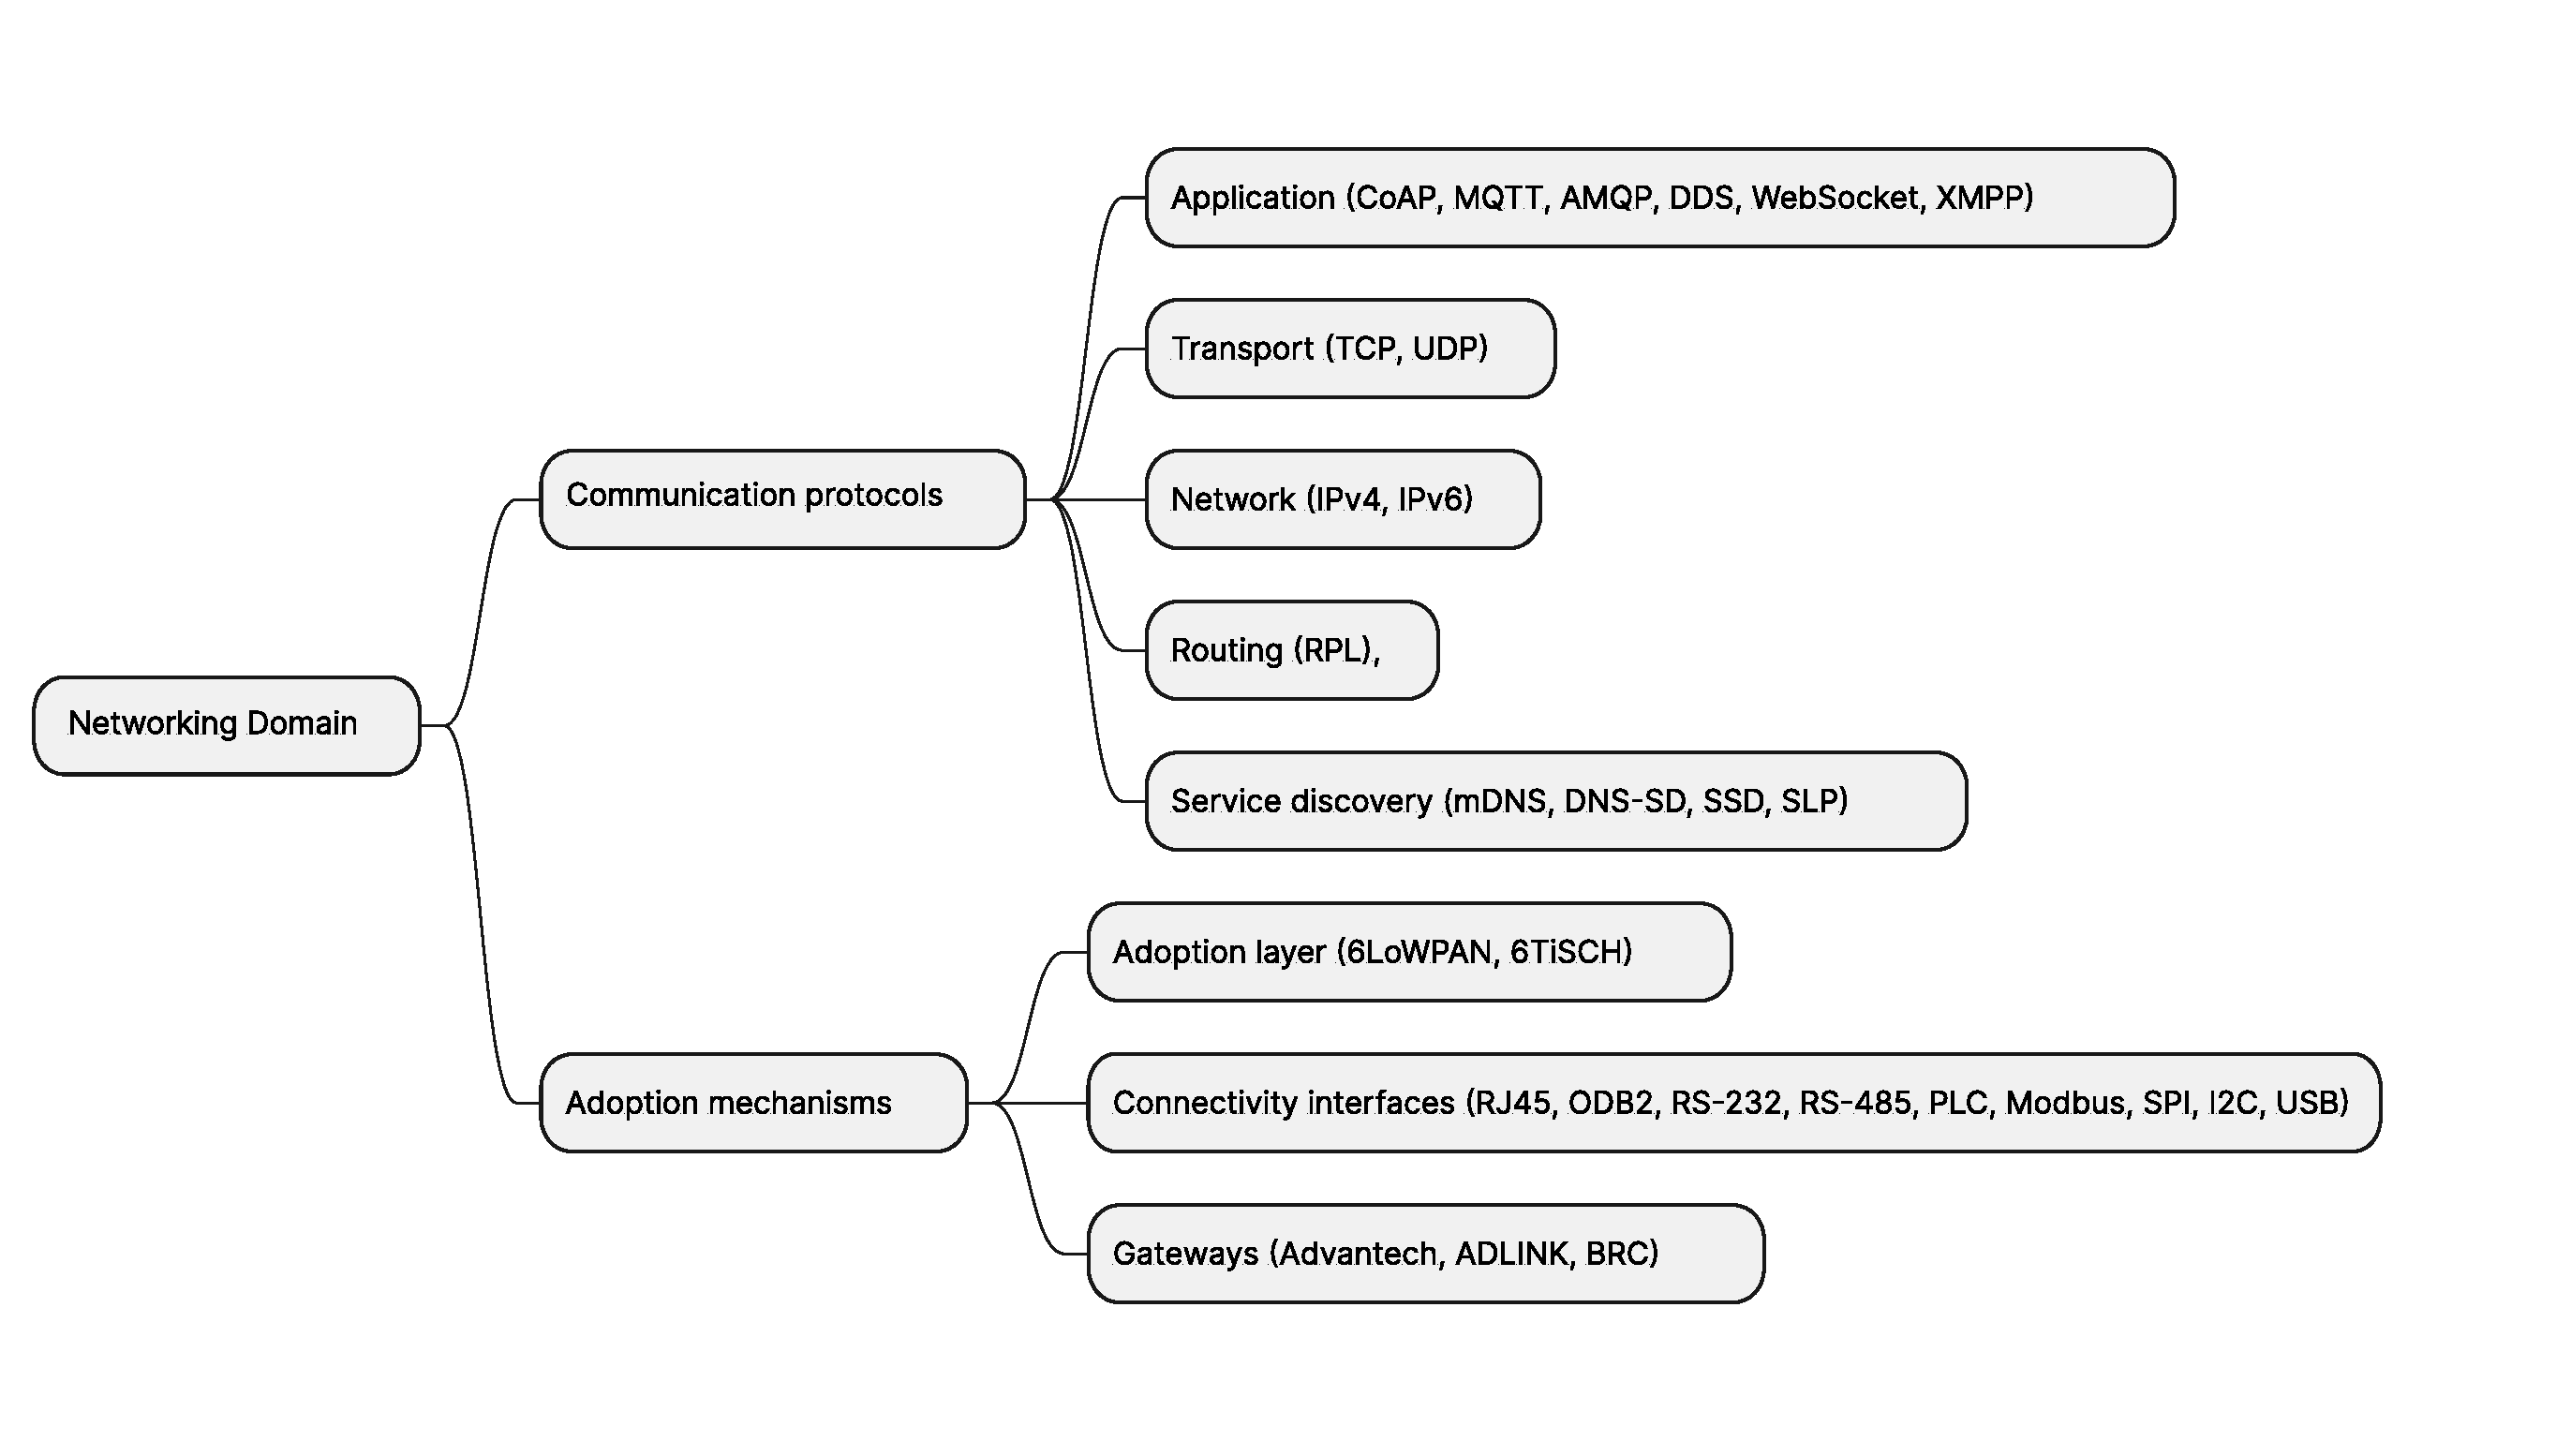
\includegraphics[width=0.9\textwidth]{./figures/IoT_network_domains.pdf}
  \caption{حوزه‌های بخش شبکه در \lr{IoT}}
  \label{fig:iotNetworkingDomains}
\end{figure}

\begin{figure}[H]
  \centering
  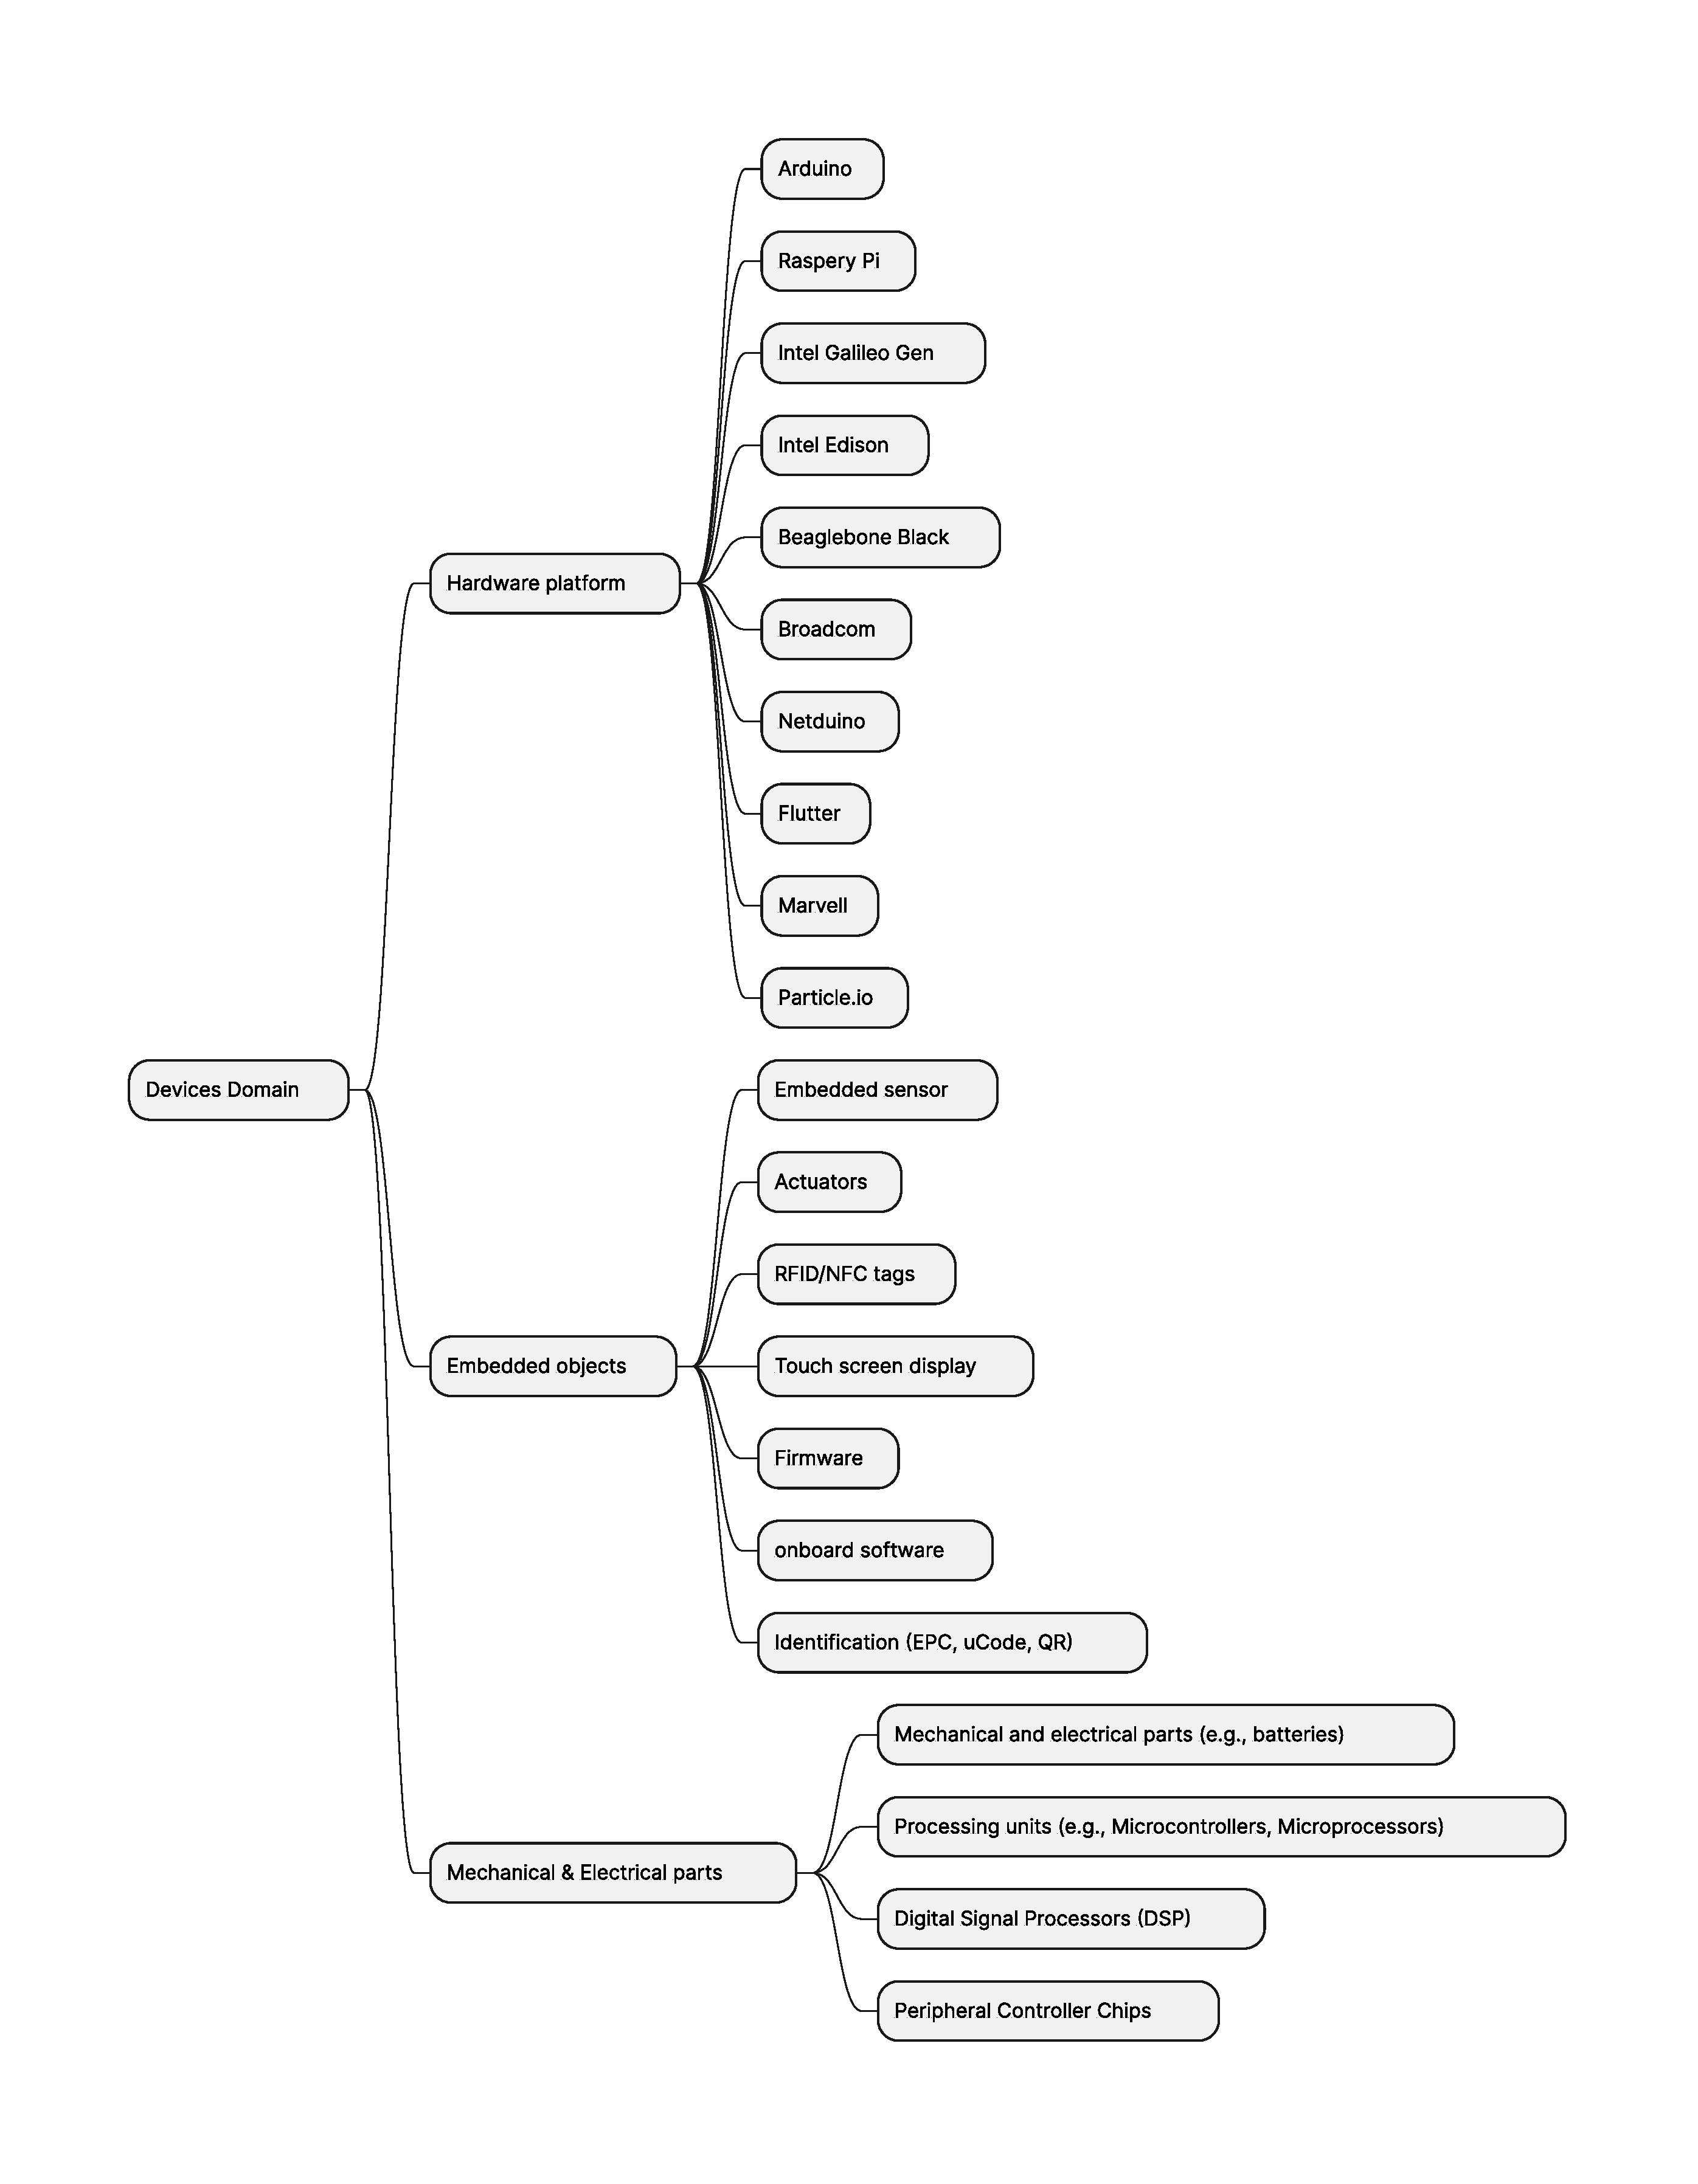
\includegraphics[width=0.9\textwidth]{./figures/IoT_devices_domains.pdf}
  \caption{حوزه‌های بخش \lr{Embedded} در \lr{IoT}}
  \label{fig:iotDevicesDomains}
\end{figure}

\subsection{عمومیت جریان داده در سیستم‌های \lr{IoT}}

عمومیت جریان داده در سیستم‌های \lr{IoT}:

\begin{itemize}
    \item دریافت داده
    \item انتقال داده
    \item پردازش داده
    \item ذخیره‌سازی داده
    \item آنالیز و معنادار کردن داده
\end{itemize}

\subsection{شاخش‌های محاسبه و ارزیابی عملکرد}

\begin{table}[H]
    \centering
    \scalebox{0.9}{
      \begin{tabular}{|>{\raggedleft\arraybackslash}p{10cm} | >{\raggedright\arraybackslash}p{5cm}|}
        \hline
        \textbf{تعاریف} & \textbf{ثابت‌ها} \\ \hline
        نرخ ورود اطلاعات & $D_{rate}$ \\ \hline
        مصرف انرژی & $E_{dev}$ \\ \hline
        تاخیر سرویس‌دهی & $T_{exe.}$ \\ \hline
        مدت زمان محاسبات & $T_{cp}$ \\ \hline
        مدت زمان ارتباطات & $T_{cm}$ \\ \hline
        مشخصات سیستم \lr{IoT} & $IoT_{sys_{sp}}$ \\ \hline
        زمان ورکلود‌ها & $t_{ws}$ \\ \hline
        تعداد دستگاه‌ها & $k$ \\ \hline
        درصد داده‌ای که در سیستم $i$ پردازش می‌شود & $\beta$ \\ \hline
        مقدار گذردهی & $\tau$ \\ \hline
        نیازمندی مشخص کارایی $P_{i_{req}}$ جایی که $P_{i}$ $i^{th}$ مقدار از کارایی است & $IoT_{sys}(P) = \{P_{i_{req}}, P_{i}\}$ \\ \hline
        مدت زمان سرویس‌دهی & $P_{i} = \langle T_{exe.}, E_{dev} \rangle$ \\ \hline
        مصرف انرژی داخلی & $E_{loc}$ \\ \hline
        انرزی مورد نیاز برای \lr{offloading} & $E_{off}$ \\ \hline
        انرژی مصرفی در زمان بیکاری & $E_{idle}$ \\ \hline
        پردازش تسک‌های داخل دستگاه & $P_L$ \\ \hline
        زمان پردازش تسک‌های داخلی & $t_L$ \\ \hline
      \end{tabular}
    }
    \caption{تعریف ثابت‌های مورد استفاده در فرمول‌ها}
    \label{table:staticAndDynamicComparison}
\end{table}

\subsubsection{فرمول شانون}

نرخ داده‌ها می‌تواند از طریق فرمول شانون محاسبه شود.

\equate{
    D_{rate} = B_{i,j} \log_{2} (1 + \frac{\lvert h_{ij} \rvert ^{2} . P_{tx}}{P_{Nj}}) 
}

\begin{itemize}
    \item $B_{ij}$: پهنای باند
    \item $h_{ij}$: بهره کانال بین دستگاه مبدا و مقصد که نشان می‌دهد سیگنال
    چگونه در مسیر بین فرستنده و گیرنده تقویت یا تضعیف می‌شود.
    \item $P_{tx}$: توان ارسال
    \item $P_{N}$: میزان نویز مقصد
\end{itemize}

کاربرد زیادی در سناریو‌هایی دارد که در آن یک ارسال کننده و یک دریافت کننده وجود
دارد.

\subsubsection{فرمول محاسبه بار سیستم یا \lr{System load}}

مجموع بار سیستم از طریق فرمول زیر بدست می‌آید:

\equate{
    D = \sum_{k = 1}^{N} D_{rate, k} \times T_{w, k}
}

\begin{itemize}
    \item $D_{rate, k}$: نرخ تولید داده توسط دستگاه \lr{IoT}
    \item $t_{w, k}$: مدت زمان ورودی در دستگاه \lr{IoT} یا به عبارتی دیگر، مدت
    زمانی که طول می‌کشد یک دستگاه \lr{IoT} ورودی را دریافت و سپس آن را پردازش و
    هندل کند.
\end{itemize}

\subsubsection{تاخیر سرویس‌دهی یا \lr{Service latency}}

مسئله تاخیر سرویس‌دهی یا \lr{service execution time ($T_{exe.}$)} مدت زمانی است
که طول می‌کشد سیستم \lr{IoT} تمام درخواست‌های پردازشی $(T_{cp})$ و ارتباطی
$(T_{cm})$ را اجرا کند \footnote{\lr{The total application exe time}}. یعنی مدت
زمان کل مصرف شده از مدت زمان سرویس یک درخواست به مدت زمان تمام تسک‌هایی که با
موفقیت پردازش شده‌اند.  بنابراین، این فاصله زمانی، بین درخواست برنامه و بدست
آوردن نتایج می‌باشد.

\subsubsection*{بخش‌هایی که زمان سرویس‌دهی دارند}

\begin{itemize}
    \item مدت زمان انتقال داده از دستگاه \lr{IoT} به زیر ساخت \lr{Fog} 
    \item مدت زمان انتقال داده از دستگاه \lr{IoT} به سرور‌های \lr{Cloud} 
    \item مدت زمان انتقال داده از \lr{Fog} به \lr{Cloud} 
    \item مدت زمان انتقال اعلانات از \lr{Cloud} به \lr{Fog} 
    \item مدت زمان انتقال اعلانات از کلاد به دستگاه‌های \lr{IoT}
    \item مدت زمان انتقال اعلانات از \lr{Fog} به دستگاه \lr{IoT}
    \item مدت زمان محاسبات در دستگاه \lr{IoT} 
    \item مدت زمان محاسبات در لایه \lr{Fog} 
    \item مدت زمان محاسبات در سرور‌های \lr{Cloud}
\end{itemize}

نکته: مدت زمانی که برای هر کاری در سیستم‌های \lr{IoT} سپری می‌شود به نوع و شیوه
پیاده‌سازی معماری دستگاه‌ها و نرم‌افزار بخش‌ها بستگی دارد و می‌تواند کاملاً
متفاوت باشند. عموماً تاخیر سرویس‌دهی بین المان‌های سیستم به صورت \lr{IoT} توزیع
شده می‌باشد و شامل دستگاه‌های اینترنت اشیا، شبکه‌ها و سیستم‌های پردازشی می‌شود.

\subsubsection*{تاخیر سرویس‌دهی}

\equate{
    T_{exe.} = T_{cm} + T_{cp}
}

مدت زمان اجرا بایستی کمتر از زمان‌بندی تسک‌ها در \lr{Fog} یا \lr{Cloud} باشد.
یعنی مدت زمان سرویس‌دهی باید کمتر از نیازمندی‌های \lr{IoT application ($T_req$)}
باشد.

برای کاهش تاخیر سرویس‌دهی از فرمول زیر بایستی پیروی کند:

\equate{
    Objective: \min (T_{exe.}) = T_{cm} + T_{cp} \leq T_{req}
}

\subsubsection{زمان ارتباطی}

\equate{
    T_{cm} = \sum_{i=1}^{N} (d_{proc} + d_{queue} + d_{trans} + d_{prop})
}    

\begin{itemize}
    \item $d_{prop}$: تاخیر پردازشی
    \item $d_{queue}$: تاخیر در صف
    \item $d_{trans}$: تاخیر انتقال
    \item $d_{prop}$: تاخیر توزیع
\end{itemize}

تاخیر مربوط به انتشار، مجموع زمان مورد نیاز برای داده، جهت ارسال از منبع به مقصد
که مبتنی بر طول لینک فیزیکی و سرعت رسانا \footnote{\lr{media}} می‌باشد.

\equate{
    d_{trans} = \frac{P_s}{R_L}
}

که در آن:

\begin{itemize}
    \item $P_s$: اندازه بسته در واحد \texttt{bits}
    \item $R_L$: سرعت لینک ارتباطی \texttt{bps}
\end{itemize}

\equate{
    d_{prop} = \frac{l_{ij}}{c}
}

\begin{itemize}
    \item $l_ij$: لینک فیزیکی
    \item $c$: سرعت توزیع و انتشار در \texttt{media}
\end{itemize}

\subsubsection{زمان پردازشی}

\equate{
    T_{cp} = T_L + \sum_{i=1}^{k} t_{offi}
}

که در آن:

\begin{itemize}
    \item $t_L$: اجرا و پردازش‌های داخلی
    \item $t_offi$: اجرا و پردازش‌های خارج از دستگاه \lr{IoT} مانند برنامه‌هایی
    که در سیستم‌های \lr{Cloud} یا \lr{Fog} مستقر شده‌اند که وظیفه پردازش تسک‌های
    \lr{Offloading} را دارند.
\end{itemize}

به بیان دیگر می‌توان آن را به صورت مدل زیر محاسبه کرد:

\equate{
    T_{cp} = t_L + t_F + t_C \\
    T_{cp} = t_L + \max_{i=1, \ldots, k} t_{F_i} + \max_{j=1, \ldots, n} t_{C_i}
}

که در آن:

\begin{itemize}
    \item $t_L$: مدت زمان پردازش‌های داخلی
    \item $t_{F_i}$: مدت زمان پردازش در نود $i^{th}$ در \lr{Fog}
    \item $t_{C_i}$: مدت زمان پردازش در سرور $i^{th}$ ابری
\end{itemize}

عموماً مصرف پردازشی بستگی به سرعت و معماری پردازنده مرکزی \lr{(CPU)}، حافظه رم
\lr{(RAM)}, سرعت حافظه ذخیره‌ساز \lr{(HDD)} یا \lr{(SSD)}، سرعت پردازنده گرافیکی
یا \lr{(GPU)} و غیره. دارد.

\subsubsection{زمان پردازش محلی $t_L$ یا زمان پردازش در هر زیر سیستم $t_{pi}$}

برای بدست آوردن زمان پردازش در هر زیر سیستم از فرمول زیر استفاده می‌شود:

\equate{
    t_{pi} = \frac{I_{CC_i}}{f_{cpu, i}}
}

\begin{itemize}
    \item $t_{pi}$: زمان پردازشی در زیر سیستم $i$
    \item $I_{CC_i}$: تعداد سایکل‌های \lr{CPU} که برای اجرای یک برنامه نیاز است.
    \item $f_{cpu, i}$: نرخ کلاک (فرکانس کاری \lr{CPU}) زیر سیستم $i$
\end{itemize}

\equate{
    t_{Pi} = t_{CPU_i} + t_{I/O_i}
}

\subsubsection{تابع محاسبه \lr{CPU time}}

مدت زمانی که در \lr{CPU} برای اجرا برنامه در نظر گرفته می‌شود به دو دسته تقسیم می‌شود:

\begin{LTR}
    \begin{itemize}
        \item \lr{User CPU time}
        \item \lr{System CPU time}: $t_{OS}$
    \end{itemize}
\end{LTR}

محاسباتی که در \lr{CPU time} انجام می‌شود خالصانه در قسمت پردازشگر مرکزی صورت
می‌گیرد و هیچ محاسبه جانبی مانند مدت زمان \lr{I/O} و مدت زمان اجرای دیگر
برنامه‌ها در نظر گرفته نمی‌شود.

\equate{
    t_{cpu_i} = \frac{I_{CC_i}}{f_{cpu_i}} + t_{OS} = I_{CC_i} \times t_{cc_i} + t_{OS}
}

حاصل این تابع معمولاً بسیار کوچک است و می‌تواند نادیده گرفته شود زیرا به سمت صفر
میل می‌کند ($t_{OS} \rightarrow 0$). به همین خاطر بیشتر روی \lr{User CPU time}
تمرکز می‌کند که توسعه‌دهنده بر روی آن کد‌های خود را اجرا می‌کند و سیستم \lr{IoT}
را راه‌اندازی می‌کند.

تابع مطرح شده بر اساس قدرت محاسباتی دستگاه $i(f_{cpu_i})$ و تعداد کلاک \lr{CPU}
برای اجرای یک برنامه ($I_{CC_i}$) می‌باشد. مقدار $f_{cpu_i}$ بر واحد \lr{(Hz)}
می‌باشد و $t_{cc_i}$ زمان چرخه کلاک است. لازم به ذکر است که $I_{CC_i}$ به نوع
دستورالعمل که شامل اندازه داده ورودی، زبان برنامه نویسی، میزان پیچیدگی الگوریتم
نرم‌افزاری مورد استفاده، و دیگر موارد می‌باشد.

بخش \lr{CPI (Clock cycles per instruction)} به عنوان میانگین تعداد چرخه کلاک است
که هر دستورالعمل به آن نیاز دارد. اگر $I_{app_j}$ تعداد دستورالعمل‌ها برای یک
برنامه باشد آن وقت $I_{CC_i}$ از طریق معادله زیر بدست می‌آید.

\equate{
    I_{CC_i} = \sum_{j=1}^{k} I_{app_j} \times CPI_{j}
}

\subsubsection{زمان پردازش محلی با توجه به اندازه داده \lr{(D)}}

\equate{
    I_{CC_i} = X \times D
}

\begin{itemize}
    \item $D$: اندازه ورودی داده بر حسب بیت
    \item $X$: شدت پردازش (تعداد چرخه‌های مورد نیاز برای هر بیت داده)
\end{itemize}

بنابراین خواهیم داشت:

\equate{
    t_{pi} = \frac{\beta_i \times D \times X}{f_{cpu, i}}
}

که در آن $\beta_{i}$ درصد داده‌‌ای است که در سیستم $i$ پردازش می‌شود.

\subsubsection{مصرف انرژی}

\subsubsection{مجموع مصرف انرژی $E_{dev}$}

برای محاسبه مصرف کل انرژی در سیستم‌های \lr{IoT} می‌توان از فرمول زیر استفاده
کرد:

\equate{
    E_{dev} = F(E_{cp}, E_{cm}, E_{idle}, E_{other})
}

\begin{itemize}
    \item $E_{cp}$: انرژی مصرف شده طی محاسبات
    \item $E_{cm}$: انرژی مصرف شده در طی ارتباطات
    \item $E_{idle}$: انرژی مصرف شده در حالت نرمال و بیکار سیستم
    \item $E_{other}$: انرژی مصرف شده توسط بقیه فرایند‌ها مانند سنسور‌ها، صفحه
    نمایش، کارت گرافیک و غیره.
\end{itemize}

یک مدل برای بررسی مصرف انرژی توسط دستگاه‌های \lr{IoT} که شامل فرایند‌های پردازشی
و ارتباطی می‌شود عبارت است از:

\equate{
    E_{dev} = E_{loc.} + E_{off.}
}

میزان انرژی مورد نیاز برای پردازش داخلی به تسک‌های داخلی وابسته می‌باشد:

\equate{
    E_{loc.} = P_L \times t_L
}

محاسبه میزان انرژی پردازشی از حاصل ضرب $I_{CC_i}$ و انرژی مصرفی \lr{CPU} به ازای
هر چرخه \lr{CPU} بدست می‌آید:

\equate{
    E_{loc.} = k \times I_{CC_i} \times f^{2}_{cpu_i} = k \times D \times X \times f^2_{cpu_i}
}

\begin{itemize}
    \item $k$: ثابتی است که به مشخصات سخت‌افزار مربوط است.
    \item $D$: اندازه داده ورودی بر مبنای \lr{bits}
    \item $X$: شدت یا داده ورودی محاسباتی
\end{itemize}

محاسبه انرژی برای انجام تسک‌های \lr{offloading} نیازمند انرژی برای ارسال داده‌ها
و دریافت نتایج آن می‌باشد که با $E_{comm}$ نمایش می‌دهند. لازم به ذکر است مدت
زمانی که طول می‌کشد سیستم نتایج را دریافت کند سیستم در وضعیت \lr{idle} باقی
مانده است. به همین صورت برای بدست آوردن مصرف انرژی برای تسک‌های \lr{offloading}
از فرمول زیر استفاده می‌شود:

\equate{
    E_{off.} = E_{cm.} + E_{idle}
}

در واقع $E_{id}$ انرژی مورد استفاده دستگاه \lr{IoT} در زمانی که دستگاه در حالت
بیکار می‌باشد. این بیکاری به منظور آن است که دستگاه \lr{IoT} در حال انتظار برای
دریافت نتیجه از سرور‌ها می‌باشد.

\equate{
    E_{idle} = P_{idle} \times t_{off} \\
    t_{off} = T_{exe.} - (t_L + T_{cm})
}

مجموع انرژی مصرفی جهت انتقال داده‌ها با انرژی مصرفی در هنگام دریافت داده‌ها ما
را به انرژی مصرفی ارتباطی می‌رساند:

\equate{
    E_{cm} = E_{tx} + E_{rx}
}

در یکی از کار‌ها \cite{huang2012close} مدلی برای مصرف انرژی نسبت به انتقال و جا
به جایی داده‌ها مطرح شده که سطوح مختلف مصرف باتری را برای \lr{uplink} و
\lr{downlink} شامل می‌شود:

\equate{
    P_{tx} = p_{u}\tau_{u} + \beta \\
    P_{rx} = p_d \tau_{u} + \beta
}

گذردهی \lr{uplink}، $\tau_u$ می‌باشد و گذردهی \lr{downlink}، $\tau_d$ است. در
حالی که $p_u$ و $p_d$ میزان انرژی مورد نیاز برای انتقال داده‌ها در \lr{uplink} و
\lr{downlink} می‌باشد. ثابت $\beta$ میزان مصرف انرژی در حالت \lr{idle} می‌باشد.
این مقادیر کاملاً به تکنولوژی ارتباطی، پروتکل‌ها و دستگاه‌هایی که روی آن برنامه
مستقر شده است وابسته می‌‌باشد. برای انتقال همزمان \lr{uplink} و \lr{downlink}
سطح انرژی می‌تواند با فرمول زیر محاسبه شود:

\equate{
    P_{trx} = p_u\tau_u + p_d\tau_d + \beta
}

نسبت معادله \lr{uplink} بر روی \lr{downlink} به همراه پهنای باند، می‌تواند فرمول
را برای محاسبه انرژی بهینه شبکه برای انتقال یک مقدار داده معین (\lr{energy per
bit}). مقدار انرژی مورد نیاز برای ارسال از طریق فرمول $E(D)_{rx}$ میزان انرژی
مورد نیاز برای دریافت داده‌ها از طریق فرمول $E(D)_{rx}$ حاصل می‌شود.

\equate{
    E(D)_{tx} = p_u + \beta\tau^{-1}_u \\
    E(D)_{rx} = p_d + \beta\tau^{-1}_d
}

مقدار داده‌هایی که بر واحد بیت توسط دستگاه‌های \lr{IoT} ارسال و دریافت می‌شوند
به ترتیب $D_{tx}$ و $D_{rx}$ می‌باشند. با در نظر گرفتن محاسبات پیشین، می‌توان در
نهایت میزان مصرف انرژی توسط دستگاه‌های \lr{IoT} را به شکل زیر بدست آورد:

\equate{
    E_{dev} = (P_L \times t_L) + (P_{tx} \times t_{tx}) + (P_{rx} \times t_{rx}) + (P_{id} \times t_{off}) \\
    E_{dev} = (P_L \times t_L) + ((p_u\tau_u + \beta) \times t_{tx}) + ((p_d\tau_d + \beta) \times t_{rx}) + (P_{id} \times t_{off}) \\
    E_{dev} = (P_L \times t_L) + ((p_u + \beta\tau^{-1}_{u}) \times D_{tx}) + ((p_d + \beta\tau^{-1}_{d}) \times D_{rx}) + (P_{id} \times t_{off})
}

یکی از مهم‌ترین چالش‌های دستگاه‌های \lr{IoT} مربوط به مصرف باتری آن‌ها می‌باشد.
در بعضی مواقع دستگاه‌های \lr{IoT} از باتری‌هایی استفاده می‌کنند که شرایط جایگزین
کردن آن‌ها وجود ندارد. هر دستگاه \lr{IoT} حتی در حالت بیکار انرژی بابت، پردازش
داده‌ها، ارسال و دریافت داده‌ها مصرف می‌کنند. انرژی موجود $E_{dev}(t)$ در طی
زمان کاهش پیدا می‌کند. به همین ترتیب انرژی باقی‌مانده $E_{dev}(r)$ یا مدت زمانی
که سیستم می‌تواند روشن بماند از طریق فرمول زیر بدست می‌آید.

\equate{
    E_{dev}(r) = E_{dev}(i) - E_{dev}(t)
}

\begin{itemize}
    \item $E_{dev}(i)$: مقدار اولیه انرژی دستگاه
\end{itemize}

مقدار باتری باقی‌مانده $T(sys)$ به میزان ظرفیت باطری یا انرژی باقی‌مانده و انرژی
مورد نیاز دستگاه برای انجام تمام سرویس‌های دستگاه، بستگی دارد. انرژی مصرفی
وابسته به قدرت مورد نیاز برای پردازش‌های داخلی $P_{cp}$ انتقال داده‌ها $P_{cm}$
و بقیه فرایند‌ها $P_{other}$ می‌باشد.

\equate{
    T(sys) = \frac{E_{dev}(r)}{P_{cp} + P_{cm} + P_{other}}
}

یکی دیگر از چالش‌های دستگاه‌های \lr{IoT} مربوط به منبع‌تغذیه آن‌ها می‌باشد. در
مواقعی که دستگاه‌های \lr{IoT} از باتری استفاده می‌کنند و به دلیل محیط‌های مختلف
شرایط به گونه‌ای است که امکان تعویض باتری وجود ندارد، محدودیت‌های باتری اغلب به
عنوان شاخص طول عمر دستگاه‌های \lr{IoT} استفاده می‌شود و می‌تواند به عنوان یکی از
مهم‌ترین معیار‌های \lr{QoS} مورد استفاده قرار گیرد. هدف اصلی در این دستگاه‌ها
این است که مصرف انرژی به حداقل برسد و طول عمر کلی سیستم به بیشترین حد ممکن.

\subsection{مدل‌های ارزیابی کارایی}

در این بخش بررسی می‌شود که چگونه می‌توان عملکرد سیستم‌های \lr{IoT} را ارزیابی
کرد وقتی چندین شاخص کلیدی عملکرد \lr{KPIs} با واحد‌ها و اهمیت‌های مختلف وجود
دارد.

\subsubsection{ارتباط بین عملکرد و ویژگی‌های زیرساخت \lr{IoT}}

عموماً عملکرد یک برنامه به ویژگی‌های زیرساخت \lr{IoT} مانند تواند محاسباتی،
تاخیر شبکه، مصرف انرژی، و غیره وابسته است. هر تغییری در زیرساخت \lr{IoT}
می‌تواند تاثیر مستقیمی بر عملکرد برنامه داشته باشد.

\subsubsection{مشکل مقایسه \lr{KPIs} مختلف}

هر \lr{KPI} مانند تاخیر شبکه، گذردهی، پهنای باند، مصرف انرژی واحد و مقیاس خاص
خود را دارد. برای مثال تاخیر بر حسب میلی‌ثانیه \lr{ms} اندازه‌گیری می‌شود و
گذردهی بر حسب \lr{mips} و مصرف انرژی بر حسب وات‌ساعت. این تفاوت در واحد‌ها باعث
می‌شود مقایسه مستقیم آن‌ها دشوار شود. علاوه‌بر مختلف بودن واحد‌ها و معیار‌ها،
برخی از \lr{KPI}ها ممکن است از اهمیت بیشتری برخوردار باشند که معمولاً به هر شاخص
وزنی یا \lr{weight} اختصاص می‌یابد.

\subsubsection{استفاده از تابع سودمندی \lr{Utility function}}

در اینجا یک تابع کابردی به نام $IoT_{sys}(p)$ وجود دارد که عملکرد سیستم \lr{IoT}
را براساس \lr{KPI}های نرمال‌شده و وزن‌دهی شده ارزیابی می‌کند. این تابع می‌تواند
برای مقایسه مدل‌های مختلف سیستم \lr{IoT} استفاده شود و مشخص کند که کدام مدل بهتر
است.

\equate{
    IoT_{sys}(p) = \sum_{i = 1}^{n} w_i \times f(p_i)
}\label{compareIoTSystems}

\begin{itemize}
    \item $n$: تعداد شاخص‌های کلیدی کارایی
    \item $(p_i)$: ارزیابی کارایی سیستم‌های \lr{IoT}
    \item $f(p_i)$: مطابقت با تابع \lr{utility} مشخص برای ارزیابی هر \lr{KPI} که
    بین دو عدد ۰ و ۱ تبدیل (نرمال‌سازی) شده است.
    \item $w_i$: وزن ضرایب برای تعیین آن که کدام \lr{KPI} در سیستم \lr{IoT} مورد
    نظر مهم‌تر می‌باشد.
\end{itemize}

به عنوان مثال، یک سیستم \lr{IoT} داریم که برای پایش سلامتی بیماران طراحی شده
است. می‌خواهیم عملکرد این سیستم را ارزیابی کنیم. در اینجا چند \lr{KPI} مهم وجود
دارد:

\begin{enumerate}
    \item زمان تاخیر یا \lr{Latency}: مدت زمانی که طول می‌کشد داده‌ها از سنسور
    به سیستم مرکزی برسند. (بر حسب میلی‌ثانیه)
    \item مصرف انرژی یا \lr{Energy consumption}: انرژی مصرف شده توسط دستگاه‌ها
    (بر حسب وات‌ساعت).
    \item درصد دسترسی یا \lr{Availability}: درصد زمانی که سیستم آنلاین و قابل
    استفاده می‌باشد. (بر حسب درصد)
    \item دقت یا \lr{Accuracy}: درصد صحت داده‌های جمع‌آوری شده از سنسور‌ها
\end{enumerate}

\subsection*{گام‌های استفاده از مدل}

\subsubsection*{نرمال‌سازی \lr{KPI}ها}

چون شاخص‌ها واحد‌های متفاوتی دارند، ابتدا باید همه مقادیر را به یک بازه یکسان به
عنوان مثال ۰ و ۱ تبدیل کنیم. این کار باعث می‌شود تا همه \lr{KPI}ها بتوانند بدون
واحد باشند. به عنوان مثال اگر زمان تاخیر بین ۰ تا ۱۰۰ میلی‌ثانیه است، مقدار ۵۰
میلی‌ثانیه به ۰/۵ نرمال‌سازی شود. یا اگر میزان دسترسی بین ۰ تا ۱۰۰ درصد است،
مقدار ۸۰ درصد به ۰/۸ نرمال‌سازی شود.

\subsection*{وزن‌دهی}

براساس اهمیت هر \lr{KPI} یک وزن $w_i$ به آن اختصاص می‌دهیم:

\begin{LTR}
    \begin{itemize}
        \item $w_1{accuracy}$ = $0.4$
        \item $w_2{latency}$ = $0.3$
        \item $w_3{energy}$ = $0.2$
        \item $w_4{availability}$ = $0.1$
    \end{itemize}
\end{LTR}

این وزن‌ها نشان‌دهنده اولویت و اهمیت \lr{KPI} مورد نظر ما برای سیستم \lr{IoT}
می‌باشد.

\subsection*{ارزیابی عمکرد سیستم مذکور}

با استفاده از این مدل همانطور که قبلاً گفته شد می‌توان سیستم‌های \lr{IoT} را با
وجود \lr{KPI}های مختلف با یکدیگر مقایسه کرد:

در فرمول \ref{compareIoTSystems} پارامتر $f(p_i)$ مقدار نرمال‌سازی‌شده هر
\lr{KPI} می‌باشد.

مقادیر \lr{KPI}های مورد نظر برای این سیستم پایش سلامت به صورت زیر می‌باشد: 

\begin{itemize}
    \item $f(p_1)$: $0.9$ دقت
    \item $f(p_2)$: $0.6$ زمان تاخیر
    \item $f(p_3)$: $0.7$ مصرف انرژی
    \item $f(p_4)$: $0.8$ میزان دسترسی
\end{itemize}

لازم به ذکر است ه مقادیر $f(p_i)$ توسط مدل‌هایی که تاکنون توضیح داده شد بدست
آمده است و سپس مقادیر آن‌ها بین ۰ و ۱ نرمال‌سازی شده است.

با توجه به مدل \ref{compareIoTSystems} خواهیم داشت:

\equate{
    (0.8 \times 0.1) + (0.7 \times 0.2) + (0.6 \times 0.3) + (0.9 \times 0.4) = 0.78
}

برای سیستم مورد نظر با توجه به مقادیری که برای \lr{KPI}های مورد نظر بدست آمده
بود مقدار $0.78$ در حقیقت مقدار مدل سیستم پایش سلامت شد. با استفاده از این مقدار
می‌توان عملکرد سیستم‌های پایش سلامت دیگر (یا دیگر سیستم‌های \lr{IoT} مربوط به آن
دامنه) را نیز به همین ترتیب ارزیابی کرد و با مقادیری که در نهایت با استفاده از
مدل \ref{compareIoTSystems} بدست می‌آید، هر کدام از آن‌ها را با یکدگیر مورد
مقایسه و \lr{Trade off} قرار داد.

دو \lr{KPI} در سیستم‌های \lr{IoT} وجود دارد که می‌تواند سطح کارایی آن‌ها را مشخص
کند. اول تاخیر در سرویس‌دهی، دوم مصرف انرژی. به همین ترتیب برای محاسبه سطح کلی
کارایی سیستم‌های \lr{IoT} از مجموع مقادیر تابع سودمندی برای هر \lr{KPI}
استفاده می‌شود:

\equate{
    IoT_{sys}(p) = w_{T_{exe}} \times f(T_{exe}) + w_{e_{dev}} \times f(E_{dev})
}

توابع $f(T_{exe.})$ و $E_{con.}$ توابع سودمندی هستند برای مدت زمان اجرا و
مصرف انرژی و در ادامه آن $w_{T_{exe.}}$ و $w_{E_{conn.}}$ وزن‌های ضریب توابع
هستند.

\subsubsection{مدل‌سازی توابع سودمندی برای هر \lr{KPI}}

در این بخش بررسی می‌کنیم که چگونه می‌توان توابع سودمندی یا \lr{Utility
functions} را برای هر \lr{KPI} مدل‌سازی کنیم. برای \lr{KPI}هایی مانند تاخیر
شبکه، مصرف انرژی، سرعت انتقال داده از توابع سیگموئیدی استفاده می‌شود که محدوده
خروجی آن‌ها بین ۰ و ۱ می‌باشد و معیار عملکرد \lr{KPI} را به صورت بی‌واحد نمایش
می‌دهد.

نکات مهم:

\begin{itemize}
    \item $f(p_t)$ یا $f(p_i \uparrow)$: برای \lr{KPI}هایی که مقدار‌‌های بیشتر
    بهتر است مانند طول عمر باتری یا گذردهی.
    \item $f(p_u)$ یا $f(p_i \downarrow)$: برای \lr{KPI}هایی که مقدار کمتر بهتر
    است مانند تاخیر یا مصرف انرژی.
\end{itemize}

\subsubsection{فرمول تابع سیگموئید}

\equate{
    f(p_i \uparrow) = L(\frac{A}{1+e^{-\alpha_k \frac{(p_i - r_i)}{z_i}}} - U) \\
    f(p_i \downarrow) = 1 - L(\frac{A}{1+e^{-\alpha_k \frac{(p_i - r_i)}{z_i}}} - U) \\
    L = \frac{1 + e^{\frac{\alpha_k \times r_i}{z_i}}}{e^{\frac{\alpha_k \times r_i}{z_i}}} . U = \frac{1}{1 + e^{\frac{\alpha_k \times r_i}{z_i}}}
}

\begin{itemize}
    \item $\alpha_k$: شیب منحنی است که حساسیت را به تغییرات \lr{KPI} نشان می‌دهد
    (شب بیشتر برابر است با تغییر سریع‌تر عملکرد).
    \item $r_i$: نقطه مرکز یا مرجع \lr{KPI} است (مثلاً یک مقدار استاندارد بهینه
    برای \lr{KPI} که \lr{IoT} باید به آن نزدیک باشد).
    \item $L$: بیشترین مقدار سودمندی
    \item $U$: کمترین مقدار سودمندی
\end{itemize}

\subsubsection{اهداف فرمول‌های سیگموئید}

\begin{itemize}
    \item برای \lr{KPI}هایی که افزایششان مطلوب است مانند گذردهی بیشتر بایستی
    $f(p \uparrow)$ را ماکزیمم کنیم.
    \item برای \lr{KPI}هایی که کاهششان مطلوب است باید $f(p \downarrow)$ را
    مینیمم کنیم.
\end{itemize}

این مدل به ما اجازه می‌دهد که عملکرد \lr{KPI}های مختلف را بدون واحد قابل مقایسه
کنیم و \lr{KPI}ها را براساس وزنی که به آن‌ها داده‌ایم مرتب کنیم و تصمیم‌گیری‌های
بهینه‌تری برای بهبود عملکرد \lr{IoT} انجام دهیم (برای مثال کدام \lr{KPI}ها بیشتر
نیاز به بهینه‌سازی دارند).

روشی که در بالا ذکر شد اندازه‌گیری انعطاف‌پذیری را برای پارامتر‌ها ارائه می‌دهد
حتی زمانی که هیچ مقدار مرجعی برای دستگاه \lr{IoT} نداشته باشیم. این مدل به دلیل
بی‌واحد بودن مقادیر به \lr{KPI} خاصی وابسته نمی‌باشد. با این روش امکان تنظیم
تابع سودمندی براساس حساسیت پارامتر‌های فردی فراهم می‌شود.

\newpage
\bibliographystyle{unsrt-fa}
\bibliography{refs.bib}
\end{document}